\documentclass[
    12pt,
    a4paper,
    english,
    brazil,
    sumario=tradicional]{abntex2}
\usepackage{lmodern}
\usepackage[T1]{fontenc}
\usepackage[utf8]{inputenc}
\usepackage{lastpage}
\usepackage{indentfirst}
\usepackage{color}
\usepackage{graphicx}
\usepackage{caption}
\usepackage{subcaption}
\usepackage{microtype}
\usepackage[brazil]{babel}
\usepackage[brazilian,hyperpageref]{backref}
\usepackage[alf]{abntex2cite}
\usepackage{multirow}
\usepackage{gensymb}
\usepackage[table]{xcolor}
\usepackage{tabulary}
\usepackage{pdfpages}

%%%% Configurações %%%%
\renewcommand{\backrefpagesname}{Citado na(s) página(s):~}
\renewcommand{\backref}{}
\renewcommand*{\backrefalt}[4]{
	\ifcase #1 %
		Nenhuma citação no texto.%
	\or
		Citado na página #2.%
	\else
		Citado #1 vezes nas páginas #2.%
	\fi}%

\setlength{\parindent}{1.3cm}
\setlength{\parskip}{0.2cm}

%%%% Constantes de autoria %%%%

\titulo{Uma solução de aprendizagem de máquina para detecção de anomalias em imagens aéreas da floresta amazônica}
\autor{Luiz Carlos A. M. Cavalcanti}
\local{Manaus}
\data{2015}
\orientador[Orientadora:]{Prof\textsuperscript{a}. Dra. Eulanda Miranda dos Santos}
\instituicao{
    PODER EXECUTIVO
    \par
    MINISTÉRIO DA EDUCAÇÃO
    \par
    UNIVERSIDADE FEDERAL DO AMAZONAS
    \par
    INSTITUTO DE COMPUTAÇÃO
    \par
    PROGRAMA DE PÓS-GRADUAÇÃO EM INFORMÁTICA
}

\preambulo{Proposta de dissertação apresentada ao Programa de Pós-graduação em Informática da Universidade Federal do Amazonas como requisito parcial para obtenção do grau de Mestre em Informática. 
Área de concentração: Visão Computacional e Robótica}

\tipotrabalho{Dissertação (Mestrado)}

%%%% Documento %%%%

\begin{document}

\imprimircapa
\imprimirfolhaderosto

\pagenumbering{roman}

\begin{folhadeaprovacao}
    \begin{center}
        {\ABNTEXchapterfont\large\imprimirautor}
        \vspace*{\fill}\vspace*{\fill}
        \begin{center}
            \ABNTEXchapterfont\bfseries\Large\imprimirtitulo
        \end{center}
        \vspace*{\fill}
    \hspace{.45\textwidth}
    \begin{minipage}{.5\textwidth}
        \imprimirpreambulo
    \end{minipage}%
    \vspace*{\fill}
    \end{center}

    Trabalho aprovado. \imprimirlocal, \today:
    \assinatura{\textbf{\imprimirorientador} \\ Orientadora}
    \assinatura{\textbf{Professor} \\ Convidado 1}
    \assinatura{\textbf{Professor} \\ Convidado 2}

    \begin{center}
        \vspace*{0.5cm}
        {\large\imprimirlocal}
        \par
        {\large\imprimirdata}
        \vspace*{1cm}
    \end{center}
\end{folhadeaprovacao}

\begin{dedicatoria}
	\vspace*{\fill}
	A dedicatória...
	\vspace*{\fill}
\end{dedicatoria}

\begin{agradecimentos}
   Os agradecimentos...
\end{agradecimentos}

\begin{epigrafe}
	\vspace*{\fill}
	\begin{flushright}
		A epígrafe...
	\end{flushright}
\end{epigrafe}

\tableofcontents*
\clearpage

\listoffigures
\clearpage

\listoftables
\clearpage

\begin{siglas}
	\item[BSD500] Berkeley Segmentation Data Set and Benchmarks 500
	\item[CENSIPAM] Centro Gestor e Operacional do Sistema de Proteção da Amazônia
	\item[CFS] Correlation-based Feature Subset Selection
	\item[IBGE] Instituto Brasileiro de Geografia e Estatística
	\item[INPE] Instituto Nacional de Pesquisas Espaciais
	\item[FSEG] Factorisation-Based Segmentation
	\item[GCE] Global Consistency Error
	\item[JPEG] Joint Photographic Experts Group
	\item[KNN] K-Nearest Neighbours
	\item[LBP-HF] Local Binary Pattern Histogram Fourier
	\item[LCE] Local Consistency Error
	\item[LIDAR] Light Detection and Ranging
	\item[OCNN] One-Class Nearest Neighbours
	\item[OC-SVM] One-Class Support Vector Machines
	\item[PDI] Processamento Digital de Imagens
	\item[RADAR] Radio Detection and Ranging
	\item[ROC] Receiver Operating Characteristic
	\item[SRM] Statistical Region Merging
	\item[SVM] Support Vector Machines
	\item[UAV] Unmanned Aerial Vehicle
	\item[VANT] Veículo Aéreo Não-Tripulado
\end{siglas}


\pagenumbering{arabic}

\begin{resumo}
    Durante o patrulhamento de crimes ambientais, o tempo de resposta é um componente muito importante no sucesso das missões. Geralmente as infrações ocorrem em lugares ermos e de difícil acesso, características que dificultam tanto o patrulhamento quanto a ação de agentes de preservação ambiental. Para aumentar a taxa de sucesso das abordagens e reduzir o risco de vidas humanas, veículos aéreos não-tripulados (VANTs) podem ser usados para cobrir grandes áreas de floresta em pouco tempo, sem que sejam percebidos por infratores, permitindo que os órgãos de patrulhamento dessas áreas possam planejar e agir com mais eficiência na repressão a esses crimes. O novo problema gerado por essa abordagem é a enorme quantidade de dados gerada durante essas missões, que muitas vezes compreendem horas de vídeo. A inspeção manual de todo esse material em busca de elementos antrópicos é muito cansativa e propensa a erros. Este trabalho apresenta uma avaliação de técnicas de segmentação de imagens, inspeção de características a serem extraídas, seguido da classificação supervisionada destes segmentos para detecção de elementos antrópicos em imagens aéreas da floresta amazônica. Além da publicação de uma base de dados com cerca de 3.000 imagens e 10.000 segmentos devidamente rotulados, o trabalho investiga diferentes estratégias para classificação de elementos antrópicos, com resultados de precisão acima de 94\% para conjuntos de classificadores unários.

    \vspace{\onelineskip}
    \noindent
    \textbf{Palavras-chaves}: aprendizado de máquina, segmentação, classificação, imagens aéreas, elementos antrópicos
\end{resumo}

\begin{resumo}[Abstract]
    During environmental crimes patrolling, the response time is a very important component for the success of the missions. Generally, infractions occur in remote and hard-access places, characteristics that hinder both the patrolling as well the action of environmental protection agents. To increase the approaches' success rate and reduce the risk of human lives, unmanned aerial vehicles (UAVs) can be used to cover large areas of forest in a short time without being perceived by offenders, allowing the patrolling organs responsible for these areas to plan and act more efficiently in the repression of such crimes. The new problem generated by this approach is the huge amount of data generated during these missions, which often includes hours of video. The manual inspection of all this material in searching for anthropic elements is very tiring and error-prone. This work presents a evaluation of image segmentation techniques, inspections of features to be extracted, followed by a supervised classification of those segments for anthropic element detection in amazon's rain forest aerial images. Besides making publicly available a dataset with more than 3,000 images and 10,000 segments labeled accordingly, this work investigates different strategies for anthropic elements classification, with results over 94\% of precision for one-classe classifiers ensembles.
    \vspace{\onelineskip}
    \noindent
    \textbf{Keywords}: machine learning, segmentation, classification, aerial images, anthropic elements
\end{resumo}


\textual

\chapter{Introdução}

Os órgãos de segurança e de patrulhamento ambiental lidam diariamente com missões de alto risco. Essas missões têm grande custo de operação e representam um perigo significativo para os agentes humanos envolvidos. Especificamente na região da floresta amazônica, a área a ser patrulhada possui uma dimensão ímpar: 11 mil quilômetros de fronteiras e 22 mil quilômetros de rios, compondo uma área total de 5.217.423 quilômetros quadrados do que é conhecido como Amazônia Legal, o que corresponde à aproximadamente 61\% do território brasileiro \cite{ibge}.

Com o intuito de minimizar os custos, aumentar a eficiência e mitigar os riscos humanos de diversos tipos de atividades, são empregados Veículos Aéreos Não-Tripulados (VANTs). Trata-se de veículos autônomos ou controlados remotamente, que têm como objetivo a agilidade e a discrição no reconhecimento de áreas isoladas ou hostis, antes que uma equipe de agentes humanos precise intervir. Essa abordagem permite que as eventuais ameaças sejam previamente identificadas, e o comando tático possa tomar as melhores decisões sobre quando e como agir na região em questão.

Os VANTs têm sido utilizados em uma miríade de missões de diferentes naturezas, com destaque para o combate a crimes em áreas de fronteira. Na região da Floresta Amazônica, os veículos podem ser utilizados no combate ao tráfico de animais, à extração ilegal de madeira e outros crimes ambientais \cite{silva:2013}.

Por acontecerem em regiões isoladas e de difícil acesso, os responsáveis por essas infrações costumam escapar antes que os agentes de segurança possam agir. A aproximação de humanos alerta os infratores, pois os veículos (barcos, helicópteros e veículos terrestres utilitários) usados na abordagem produzem sons bastante perceptíveis nesses ambientes. Por esses motivos, os VANTs representam uma boa alternativa para possibilitar flagrantes e o planejamento tático dessas missões.

Equipados com câmeras de diversos tipos e alcances, esses veículos são capazes de gerar muitas horas de vídeo a cada missão, tornando a análise simultânea ou posterior do material gerado um grande esforço para as pessoas responsáveis pelo planejamento tático, presentes em salas de controle para onde os vídeos são transferidos ao vivo, ou analisados posteriormente.

\section{Motivação}

A quantidade maciça de dados gerados pelos VANTs leva à necessidade de desenvolvimento de procedimentos capazes de avaliar essa grande quantidade de material e identificar os prováveis pontos de interesse. Uma solução computacional capaz de fazer tal análise seria importante por possibilitar a rápida avaliação do material gerado por uma operação, ou mesmo para que uma quantidade menor de profissionais seja necessária para o acompanhamento em tempo real de diversos VANTs em uma mesma missão. Isso cria uma demanda para a filtragem e classificação desses dados em informações ou alertas relevantes aos agentes humanos que supervisionam esses equipamentos.

Ao provar a eficiência de uma implementação automatizada dessa classificação, um significativo aumento pode ser alcançado na qualidade e agilidade da detecção de elementos antrópicos em ambientes silvestres, bem como na redução da margem de erro dos agentes humanos envolvidos. A detecção de elementos antrópicos refere-se à identificação de objetos estranhos ao padrão normal do ambiente silvestre, oriundo de atividades humanas.

Através de processamento de imagens digitais e reconhecimento automático de padrões, é possível avaliar o material com maior rapidez, e sinalizar os pontos de possível interesse dos profissionais que acompanham as missões.

Baseando-se em elementos antrópicos encontrados nas imagens aéreas de regiões silvestres, áreas com relativa previsibilidade de paisagem, é possível buscar padrões e reconhecer ameaças ou interesses que possam passar despercebidos por olhos humanos, especialmente em um material com extensão de horas. Tais elementos antrópicos incluem acampamentos de caçadores, pistas clandestinas, estradas, embarcações, ou seja, indícios de presença humana em áreas de selva.

Até a conclusão desta dissertação, não foi possível encontrar na literatura trabalhos que abordassem a detecção de elementos antrópicos em regiões de floresta amazônica, tampouco que utilizassem imagens aéreas da região obtidas por aeronaves. Diante desse contexto, este projeto propõe o uso de técnicas de processamento digital de imagens e de aprendizagem de máquina para detectar elementos antrópicos em imagens obtidas por veículos aéreos, de uma região da Floresta Amazônica.

\section{Objetivos}

\subsection{Geral}

Este trabalho tem como objetivo propor uma abordagem utilizando processamento digital de imagens (PDI) e aprendizagem de máquina para o problema de detecção automática de elementos antrópicos em imagens aéreas da floresta amazônica. A intenção é demonstrar que a identificação automática destes elementos pode trazer benefícios, em especial agilidade, ao processo que hoje é completamente dependente de agentes humanos, e produzir elevadas taxas de acerto.

\subsection{Específicos}

\begin{itemize}
    \item Organizar uma base de dados de imagens devidamente rotuladas que sirva de referência para futuros estudos desta problemática.
    \item Investigar e definir métodos para segmentação de imagens aéreas de floresta amazônica.
    \item Investigar e definir métodos para extração e seleção de características mais adequadas ao problema em questão.
    \item Apontar o melhor conjunto de técnicas para a detecção de elementos antrópicos em imagens aéreas da floresta amazônica.
\end{itemize}

\section{Organização do Documento}

O restante deste documento está organizado da seguinte forma: no capítulo \ref{cap:fundamentacao} discorremos sobre a fundamentação teórica necessária para o entendimento do trabalho proposto. No capítulo \ref{cap:trabalhos} os trabalhos relacionados são apresentados, com ordem e critérios descritos neste mesmo capítulo. Uma comparação das referências também é feita. No capítulo \ref{cap:metodologia} é descrita a metodologia que será empregada no desenvolvimento deste trabalho de pesquisa. No capítulo \ref{cap:experimentos} são apresentadas a base de dados, sua preparação e a descrição dos experimentos realizados, com os resultados alcançados. Por fim, no capítulo \ref{cap:conclusao} uma conclusão para o trabalho é apresentada, consolidando os resultados dos experimentos e apontando possibilidades para trabalhos futuros.


\chapter{Fundamentação Teórica}\label{cap:fundamentacao}

Neste capítulo são discutidos os conceitos básicos ao entendimento deste trabalho, abrangendo processamento digital de imagens, segmentação de imagens, aprendizagem de máquina, extração de características e avaliação de desempenho dos métodos utilizados.

\section{Processamento Digital de Imagens}

Uma imagem pode ser definida por uma função bidimensional, $f(x,y)$, onde $x$ e $y$ são coordenadas espaciais de um plano, e a amplitude de $f$ para um par de coordenadas $(x,y)$ é chamada de intensidade da imagem naquele ponto. Quando $x$, $y$ e a amplitude de valores de $f$ representam quantidades finitas e discretas, podemos chamar a imagem de imagem  digital. A linha de pesquisa de processamento digital de imagens se refere ao processamento digital dessas imagens através de um computador digital \cite{gonzalez:2002}.

Uma imagem digital é composta por um número finito de elementos, cada um com um valor ($f$) e localização ($x$ e $y$) particulares. Estes elementos são chamados de elementos da imagem ou \textit{pixels}, do inglês \textit{picture elements}.

Ainda de acordo com \citeonline{gonzalez:2002}, o interesse em processamento digital de imagens advém de duas principais áreas de aplicação: melhoramento de informações pictóricas para interpretação humana; e processamento de imagens para armazenamento e transmissão de dados, e representação para percepção de máquinas autônomas. 

Em muitos problemas, como o de interpretação de imagens por uma máquina, é comum que algum processo de segmentação seja realizado, e as imagens sejam divididas em regiões para processamento posterior.

\subsection{Segmentação de Imagens}

O processo de segmentação subdivide uma imagem em suas várias regiões ou objetos. O nível em que a subdivisão é feita depende do problema a ser resolvido, ou seja, a segmentação deve parar quando os objetos de interesse de uma aplicação forem isolados. Por exemplo, na inspeção automática de uma linha de montagem de produtos eletrônicos, o interesse reside em analisar imagens dos produtos com o objetivo de determinar a presença ou ausência de anomalias específicas, como componentes faltando ou conexões quebradas. Não há sentido em continuar segmentando além do nível de detalhes necessário para a identificação destes elementos.

Segmentação de imagens é um dos problemas mais difíceis em processamento digital de imagens \cite{gonzalez:2002}. Algoritmos de segmentação geralmente se baseiam em uma das duas propriedades básicas de valores de intensidade dos pixels: descontinuidade e similaridade. Na primeira propriedade, a abordagem é particionar a imagem baseando-se em mudanças abruptas na intensidade dos pixels, como as bordas. A segunda categoria se baseia no particionamento de uma imagem em regiões que são similares de acordo com um critério em particular, que pode ser coloração, textura, entre outros.

Neste trabalho, conforme será descrito no capítulo \ref{cap:metodologia}, testamos uma série de atributos para determinar a melhor forma de segmentar as regiões das imagens aéreas da floresta amazônica, como uma das etapas da pesquisa de detecção de elementos antrópicos. Muitas vezes, técnicas de segmentação de imagens não são suficientes para isolar ou detectar componentes específicos na coleção de imagens. Trabalhos recentes têm utilizado, com frequência, algoritmos de aprendizagem de máquina para resolver este problema.


\subsection{Avaliação de segmentação}\label{sec:avaliacaopdi}

Para avaliar a qualidade de uma segmentação, em primeiro lugar é preciso aferir a validade da base de dados de segmentações manuais (\textit{ground-truth}), demonstrando que segmentações de uma mesma imagem feitas por diferentes indivíduos são consistentes. Em um segundo momento, é preciso avaliar os algoritmos de segmentação de forma objetiva.

O problema em mensurar a consistência entre duas segmentações é que não há uma única segmentação possível para uma imagem. Duas pessoas podem segmentar uma imagem de forma significativamente diferente por terem uma percepção diferente da cena, ou ainda, por usar diferentes granularidades na segmentação, caso exemplificado na figura \ref{fig:granularidade}.

\begin{figure}[h]
  \centering
  \begin{subfigure}[b]{0.3\textwidth}
    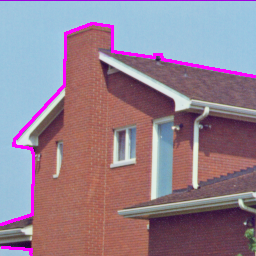
\includegraphics[width=\textwidth]{imgs/granularidade_1}
  \end{subfigure}%
  ~
  \begin{subfigure}[b]{0.3\textwidth}
    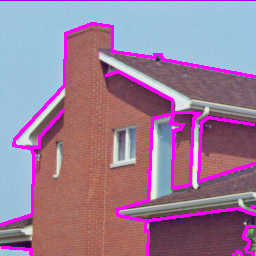
\includegraphics[width=\textwidth]{imgs/granularidade_2}
  \end{subfigure}%
  ~
  \begin{subfigure}[b]{0.3\textwidth}
    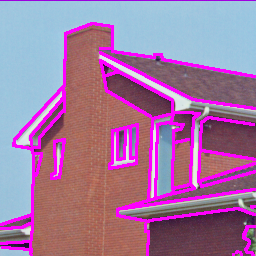
\includegraphics[width=\textwidth]{imgs/granularidade_3}
  \end{subfigure}%
  \caption{A mesma imagem segmentada de forma consistente, mas com diferentes granularidades de segmentação}
  \label{fig:granularidade}
\end{figure}

Quando a diferença entre duas segmentações advém de uma diferença de percepção da cena, é esperado que o erro seja grande e que as segmentações sejam consideradas inconsistentes. Quando a diferença é de granularidade, uma segmentação pode ser considerada apenas um refinamento da outra, portanto, o erro deve ser baixo ou até zero \cite{martin:2001}.

Segmentação de imagens é simplesmente a divisão de pixels de uma imagem em conjuntos (segmentos). Uma possível medida de erro tem como entrada duas segmentações, $S_1$ e $S_2$, e tem como saída um valor real no intervalo $[0...1]$, onde $0$ significa ausência de erros de segmentação.

Ainda de acordo com o trabalho de \citeonline{martin:2001}, é necessário utilizar medidas que sejam lenientes com o refinamento de granularidade entre duas segmentações de uma mesma imagem. Entende-se que se os pixels de um segmento podem ser considerados um subconjunto adequado de um outro segmento, trata-se de um refinamento e o erro deve ser zero. Se não existe relação de subconjunto entre os segmentos, as regiões devem ser consideradas inconsistentes e o erro deve ser significativo.

Se $R(S,p_i)$ é o conjunto de pixels correspondentes a uma região na segmentação $S$ que contém o pixel $p_i$, onde $\setminus$ denota o conjunto complementar, o erro de refinamento local é definido por:

\begin{equation}
	\displaystyle E(S_1,S_2,p_i) = \frac{|R(S_1,p_i) \setminus R(S_2,p_i)|}{|R(S_1,p_i)|}
\end{equation}


A partir desta relação, \citeonline{martin:2001} define duas métricas de erro de segmentação: Erro de Consistência Global (Global Consistency Error, ou GCE) e Erro de Consistência Local (Local Consistency Error, ou LCE):

\begin{equation}
	\displaystyle GCE(S_1,S_2) = \frac{1}{n} min \biggl\{ \sum_{i} E(S_1,S_2,p_i), \sum_{i} E(S_2,S_1,p_i) \biggr\}
\end{equation}

\begin{equation}
	\displaystyle LCE(S_1,S_2) = \frac{1}{n} \sum_{i} min \biggl\{ E(S_1,S_2,p_i), E(S_2,S_1,p_i) \biggr\}
\end{equation}

Uma vez que $LCE \geq GCE$ entre segmentações de uma mesma imagem, é correto afirmar que $GCE$ é uma medida mais rígida que $LCE$. Além dos casos em que uma segmentação é um refinamento de outra, há ainda dois casos em que o erro de segmentação pode ser zero: quando os segmentos são compostos por apenas um pixel cada ou quando toda a imagem é composta de apenas um segmento.

\section{Aprendizagem de máquina e reconhecimento de padrões}

Conforme \citeonline{alpaydin:2010}, aprendizagem de máquina é uma área da inteligência artificial que estuda métodos computacionais, a fim de obter um determinado conhecimento específico através de experiências. A aplicação prática de aprendizado de máquina inclui o processamento de linguagem natural, diagnósticos médicos, detecção de intrusos, entre outros. Um sistema de aprendizado tem a função de analisar informações e generalizá-las, para a extração de novos conhecimentos.

Segundo \citeonline{russell:2010}, os tipos de aprendizagem podem ser classificados de acordo com o tipo de \textit{feedback} que recebem do ambiente:

\begin{itemize}
    \item Aprendizagem não-supervisionada: o agente aprende padrões na entrada, embora não seja fornecido nenhum \textit{feedback} explícito. A tarefa mais comum de aprendizagem não-supervisionada é o agrupamento, ou seja, a detecção de grupos de exemplos de entrada potencialmente úteis.
    \item Aprendizagem por reforço: também conhecida como aprendizagem semi-supervisionada. O agente aprende a partir de uma série de reforços - recompensas ou punições.
    \item Aprendizagem supervisionada: o agente observa alguns exemplos de pares de entrada e saída, e aprende uma função que faz o mapeamento da entrada para a saída.
\end{itemize}

Os problemas de aprendizagem podem ainda ser divididos de acordo com o tipo de saída que demandam:

\begin{itemize}
	\item Problemas de classificação: quando a saída esperada para o problema é uma classe ou categoria, ou seja, um valor discreto;
	\item Problemas de regressão: quando a saída esperada para o problema é um valor numérico, normalmente contínuo.
\end{itemize}

Um problema de classificação, ou seja, um problema em que o objetivo é atribuir corretamente classes discretas (rótulos) aos exemplos de dados, consiste na determinação de regras e posterior classificação desses exemplos. Este conjunto de regras é criado por um classificador, que recebe como entrada um vetor de características e oferece como saída uma classe resultante para a instância que as características descrevem, conforme pode ser visto na figura \ref{fig:classificador}.

\begin{figure}[h!]
  \centering
  
\includegraphics[width=0.7\textwidth]{imgs/classificador}
  \caption{Representação de classificador como uma função de bloco}
  \label{fig:classificador}
\end{figure}

Os tipos de classificadores utilizados neste trabalho serão discutidos com mais detalhes na seção \ref{sec:classificacao}.

Para composição do modelo de aprendizagem, uma base de dados de treinamento é utilizada. Esta base deve possuir uma quantidade significativa e com boa representatividade das classes envolvidas no problema. Normalmente se usa uma parte da base de dados de treinamento para validação do modelo de aprendizado (validação cruzada) ou mesmo uma base de dados diferente (base de testes ou validação), para que indicadores de qualidade do modelo possam ser avaliados. A seção \ref{sec:avaliacao} discorre sobre os métodos de avaliação utilizados neste trabalho.

Técnicas de aprendizagem de máquina podem ser utilizadas para encontrar padrões em diversos domínios, inclusive em imagens. É neste ponto que a linha de pesquisa de aprendizagem de máquina, advinda da área de inteligência artificial, se encontra com a linha de pesquisa de reconhecimento de padrões, advinda da área de processamento de sinais. Segundo \citeonline{jain:1989}, o fluxo padrão para soluções de reconhecimento de padrões consiste em três etapas:

\begin{enumerate}
    \item Filtragem e pré-processamento da entrada;
    \item Extração e seleção de características;
    \item Classificação.
\end{enumerate}


\subsection{Filtragem e Pré-processamento}

A etapa de filtragem e pré-processamento é responsável pela escolha e montagem da base de dados que será usada no processo de aprendizagem. A base deve conter uma quantidade significativa de exemplos de todas as classes envolvidas no problema.

Em aprendizado relacionado a imagens, essa etapa é comumente a responsável por normalizar e salientar as características desejadas nas amostras (realce de imagens, filtragem, etc). Exemplos irrelevantes, distorcidos ou repetidos também são eliminados durante a filtragem. O objetivo principal desta etapa é preparar a base de dados para as etapas seguintes.


\subsection{Extração de Características}

A extração de características é feita selecionando os atributos oriundos dos dados (imagens, no trabalho em questão), a fim de encontrar as características úteis para o processo de reconhecimento. Essa etapa é crítica ao sucesso do aprendizado, uma vez que bons algoritmos de aprendizado só obtêm êxito com um bom conjunto de características relevantes ao problema.

Em projetos que envolvem classificação de imagens, uma gama de atributos pode ser extraída, e podem ser descritos pelo nível da informação que representam. Nesta etapa há uma forte contribuição da linha de pesquisa de processamento digital de imagens \cite{gonzalez:2002}, que descreve filtragens, transformações e outras técnicas capazes de extrair informações sobre uma imagem ou pedaços dela.

Segundo \citeonline{nixon:2008}, informações de baixo-nível como bordas, histogramas de intensidade e coloração, são úteis para o reconhecimento de padrões em imagens, assim como características de níveis mais altos, como texturas, transformadas de Hough e extração de regiões conectadas.

O produto desta etapa é a representação de cada exemplo da base de dados em um vetor de características, de forma que possa ser usado por um ou mais classificadores em uma etapa posterior.


\subsection{Classificação}\label{sec:classificacao}

Nesta etapa, todas as amostras de treinamento são classificadas e um modelo de aprendizado é gerado. Posteriormente ao processo de aprendizado, é nesta mesma etapa que as amostras não classificadas receberão uma classe dentre as envolvidas no problema. É neste momento que podemos comparar o desempenho de diferentes algoritmos de aprendizado para o conjunto de características escolhido para representar o problema.

Pode-se também usar múltiplos classificadores, ao invés de apenas um. Esta abordagem é chamada de sistemas com múltiplos classificadores (do inglês \textit{multiple classifier systems}), também chamados de \textit{ensemble} de classificadores, os quais podem ser compostos por classificadores do mesmo tipo ou de diferentes algoritmos de classificação. 

Existe uma grande variedade de algoritmos de aprendizagem de máquina propostos na literatura. Alguns dos mais utilizados são: classificadores estatísticos, redes neurais artificiais, árvores de decisão, máquinas de vetores de suporte (SVM), k vizinhos mais próximos (KNN), etc \cite{jain:1989}.

Amplamente utilizadas em algoritmos de classificação, as árvores de decisão são representações simples do conhecimento e um meio eficiente de construir classificadores que predizem classes baseadas nos valores de atributos de um conjunto de dados. As árvores de decisão consistem de nodos que representam os atributos; de arcos, provenientes destes nodos e que recebem os valores possíveis para estes atributos; e de nodos folha, que representam as diferentes classes de um conjunto de treinamento. Classificação, neste caso, é a construção de uma estrutura de árvore, que pode ser usada para classificar corretamente todos os objetos do conjunto de dados da entrada.

A partir de uma árvore de decisão é possível derivar regras. As regras são escritas considerando o trajeto do nodo raiz até uma folha da árvore. Estes dois métodos são geralmente utilizados em conjunto. Devido ao fato das árvores de decisão tenderem a crescer muito, de acordo com algumas aplicações, elas são muitas vezes substituídas pelas regras. Isto acontece em virtude das regras poderem ser facilmente modularizadas. Uma regra pode ser compreendida sem que haja a necessidade de se referenciar outras regras.

Uma árvore de decisão tem a função de particionar recursivamente um conjunto de treinamento, até que cada subconjunto obtido deste particionamento contenha casos de uma única classe. Para atingir esta meta, a técnica de árvores de decisão examina e compara a distribuição de classes durante a construção da árvore. O resultado obtido, após a construção de uma árvore de decisão, são dados organizados de maneira compacta, que são utilizados para classificar novos casos. A árvore de decisão não presume nenhum modelo estatístico a priori, sendo a divisão do espaço de atributos feita de acordo com as amostras provenientes do treinamento.

O algoritmo KNN (K-Nearest Neighbours, ou K vizinhos mais próximos) \cite{cover:1967} é um método de classificação baseado na proximidade de amostras de treino no espaço de características. É considerado um dos mais simples algoritmos de aprendizagem de máquina.

O processo de treinamento para esse algoritmo consiste em armazenar o vetor de característica e rótulos (classes) de cada amostra de treinamento em um espaço n-dimensional, onde n é o número de características de cada amostra. No processo de classificação de amostras não-rotuladas, a amostra é simplesmente projetada no espaço e é classificada de acordo com as k amostras mais próximas.

Quando k = 1, a amostra é simplesmente classificada de acordo com o rótulo de seu vizinho mais próximo no espaço de características. Quando k é maior que 1, a classificação se dá por um esquema de votação, onde a classe com as amostras vizinhas mais numerosas é considerada como a classe da amostra. Por essa razão, em problemas bi-classe como o apresentado neste artigo devem possuir um k ímpar, para evitar empates. Em problemas multi-classe, ou seja, com mais de duas classes possíveis, empates podem acontecer mesmo considerando um número ímpar de vizinhos, de maneira que uma forma de desempate deve ser definida na implementação do algoritmo.

Diversas formas de calcular a distância entre duas amostras $a$ e $b$ em um espaço n-dimensional podem ser utilizadas no kNN, dentre elas a distância Euclidiana, representada pela fórmula \ref{eq:euclides}, onde $n$ é o número de dimensões.

\begin{equation}
	\displaystyle d(a,b) = ||a - b|| = \sqrt{(a - b)*(a -b)} =
	\displaystyle \sqrt{\sum_{i=1}^{n}(a_i - b_i)^2}
\label{eq:euclides}
\end{equation}

As máquinas de vetores de suporte, ou SVM (\textit{Support Vector Machines}) são classificadores baseados na teoria de aprendizagem estatística proposta por \cite{vapnik:1995}. A teoria é baseada em uma forte fundamentação matemática para estimação de dependências e previsão do aprendizado a partir de conjuntos de dados finitos. 

Um modelo SVM é a representação das amostras como pontos em um espaço n-dimensional (onde n é o tamanho do vetor de características) de tal forma que as amostras de diferentes classes sejam divididas por um plano de separação que maximiza a distância entre essas classes. Isso se deve ao fato de que o plano de separação possui a maior distância possível às amostras mais próximas entre as classes, o que ajuda a diminuir o erro de generalização (\textit{over-fitting}) do classificador.

A principal vantagem do classificador SVM é seu bom desempenho em conjuntos de dados que possuem muitos atributos, mesmo quando há poucas amostras de treino. No entanto, suas desvantagens são a baixa velocidade e alto consumo de recursos durante as fases de treinamento, assim como a complexidade de parametrização de suas funções \textit{kernel}. As amostras de teste são classificadas ao serem posicionadas no espaço de características e avaliadas em que lado da superfície de separação elas se encontram, como mostrado na figura \ref{fig:svm}.

\begin{figure}[h!]
  \centering
  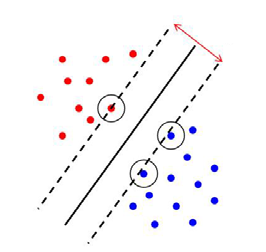
\includegraphics[scale=0.5]{imgs/svm}
  \caption[Máquina de vetores de suporte]{Amostras em um espaço bidimensional (pontos coloridos) separadas por um hiperplano apoiado por vetores de suporte (setas vermelhas), maximizando a distância entre as amostras mais próximas entre as classes (pontos circulados)}
  \label{fig:svm}
\end{figure}

Há um grupo de algoritmos de aprendizado de máquina que se baseiam em raciocínio probabilístico, especialmente sob o viés bayseano. De acordo com \citeonline{mitchell:1997}, o raciocínio bayesiano é baseado na presunção de que as quantidades de interesse são governadas pela distribuição das probabilidade e que decisões ótimas podem ser tomadas a partir da análise destas probabilidades em conjunto com os dados observados.

O teorema de Bayes estabelece a relação entre uma probabilidade condicional e sua probabilidade inversa. A equação \ref{eq:teoremaDeBayes}, conhecida como regra de Bayes, permite calcular a probabilidade de um evento (A) dado que outro evento aconteceu (B).

\begin{equation}
	\displaystyle P(A|B) = \frac{P(B|A) P(A)}{P(B)}
\label{eq:teoremaDeBayes}
\end{equation}

A probabilidade \textit{a priori}, ou seja, a probabilidade isolada de que um evento $A$ aconteça é expressa por $P(A)$. A probabilidade \textit{a posteriori} de um evento $A$ dado que ocorreu também um evento $B$ é expressa por $P(A|B)$.

Dentre as técnicas de inspiração probabilística, se destaca por sua simplicidade a \textit{Naive Bayes}. Apresentada por \citeonline{john:1995}, esta família de algoritmos presume uma forte independência entre as variáveis do vetor de características, por isso é ganhou a alcunha de Bayes Ingênuo (do inglês \textit{Naive Bayes}).

Segundo \citeonline{russell:2010}, os valores de máxima probabilidade de cada classe de acordo com as variáveis do vetor de características é encontrado. Uma vez que um modelo é gerado desta maneira, as futuras amostras podem ser classificadas de acordo com as mesmas probabilidades. Dado que o vetor de características das amostras é dado por $x_1, x_2,...,x_n$, a probabilidade de cada classe C é expressa pela equação \ref{eq:probabilidadeNaiveBayes}. A família de algoritmos \textit{Naive Bayes} tende a ser bastante robusta em face a dados ruidosos ou faltantes.

\begin{equation}
	\displaystyle P(C|x_1,x_2,...,x_n) = P(C) \prod_{i}{P(x_i|C)}
\label{eq:probabilidadeNaiveBayes}
\end{equation}


O algoritmo \textit{Random Forest}, introduzido por \citeonline{breiman:2001} , é um \textit{ensemble} de classificadores de árvore de decisão. Na fase de treinamento, um número determinado de árvores é gerado utilizando um subconjunto pseudo-aleatório do vetor de característica completo utilizado no problema. Tanto o número de árvores quanto a quantidade de atributos utilizados por cada árvore pode ser determinado pelo usuário do algoritmo.

Uma vez que a base de treinamento foi utilizada para gerar os modelos das árvores de decisão, estes mesmo modelos podem ser utilizados para classificar novas amostras do problema. Preferencialmente todas as árvores geradas são envolvidas na classificação, cada uma chegando à sua própria conclusão sobre a classe da amostra apresentada. Cada árvore tem um ``voto'', que é contabilizado para a definição da classe mais votada, que é então escolhida como a classe da amostra. Esta técnica de soma de votos é conhecida como \textit{polling}.

A principal vantagem deste algoritmo é a eliminação de \textit{overfitting}, problema bastante comum quando se utiliza árvores de decisão de forma tradicional. Uma exposição mais detalhada acerca de \textit{overfitting} é feita na seção \ref{sec:avaliacao}.

O trabalho de \citeonline{breiman:2001} ainda afirma que a taxa de erro de um modelo de aprendizado criado com \textit{Random Forest} está relacionada a dois fatores: a correlação entre quaisquer duas árvores geradas no modelo e a ``força'' de cada árvore gerada, ou seja, o quão precisa ela é em relação ao modelo geral. À medida que a correlação entre árvores cresce, também cresce a taxa de erro do modelo final. Quanto menor for a taxa de erro de uma árvore individual, mais ``forte'' é considerado o classificador, e por consequência, mais baixo é a taxa de erro do modelo.

Reduzir o número de variáveis do vetor de características a ser utilizado em cada árvore reduz a correlação entre árvores e também reduz a ``força''da árvore. Incrementar este número de variáveis incrementa a correlação e a ``força'' da árvore. A parametrização do algoritmo deve se preocupar em encontrar o número de variáveis do vetor de característica que melhor minimize a correlação e maximize a ``força'' das árvores do modelo.

Há um grupo de algoritmos em aprendizagem de máquina que tem como objetivo a detecção de anomalias a partir de um modelo formado por apenas uma classe. Neste tipo de problema, a base é normalmente composta por uma única classe (conhecida como classe alvo, ou \textit{target}) e o modelo gerado é supostamente capaz de determinar se novas amostras do problema pertencem à classe alvo ou se tratam de anomalias ou novidades (\textit{outliers}). Estes algoritmos são comumente chamados de detectores de anomalias ou novidades (\textit{novelty detection} ou \textit{outlier detection}).

Em geral, algoritmos de detecção de anomalias podem ser utilizados para resolução de problemas com múltiplas classes. A estratégia consiste em treinar um classificador deste tipo para cada classe do problema. Diversas técnicas para apuração dos resultados podem ser utilizadas, tais como votação (\textit{voting} ou \textit{polling}), onde cada classificador tem um voto que é computado com um peso e levado em consideração na classificação final; ou bagging (abreviação do termo inglês \textit{Bootstrap aggregating}), que se utiliza da combinação do resultado de classificação de conjuntos de dados de treinamento selecionados aleatoriamente, com o objetivo de reduzir a variância e o \textit{overfitting}, discutidos com mais detalhes na seção \ref{sec:avaliacao}.

Uma variante do SVM denominada OC-SVM (acrônimo em inglês para \textit{One Class Support Vector Machines}) foi introduzida por \citeonline{scholkopf:1999} com a finalidade de adaptar o robusto algoritmo de \citeonline{vapnik:1995} para problemas de detecção de anomalias. Este é, na verdade, uma expansão da aplicação da técnica de SVM para dados não-rotulados.

A ideia central é que uma função \textit{kernel} de base radial é utilizado para comportar as amostras da classe alvo, de forma a medir a possibilidade de anomalias futuras de acordo com a distância destas mesmas amostras em relação à hiperesfera de separação descrita pela função \textit{kernel}. Em uma problema com múltiplas classes e classificadores OC-SVM, costuma-se usar uma estratégia de votação com pesos para determinação da classe da amostra.

Outros métodos tradicionais em problemas multi-classe também podem ser usados como classificadores para detecção de anomalias. Variações de KNN como o OCNN (\textit{One-Class Nearest Neighbour}) ou de árvores de decisão como o REPTree são comumente utilizados nesta abordagem, utilizando diversas estratégias para determinação final das classes das novas amostras.

O trabalho de \citeonline{hadjadji:2014} apresenta uma modelo para conjuntos de classificadores de anomalias em que diversos algoritmos e estratégias diferentes podem ser utilizados em conjunto para um mesmo problema de aprendizagem. Isto possibilita um grau de liberdade elevado na escolha desses algoritmos e estratégias para problemas multi-classe.

Tanto durante o desenvolvimento de uma solução, quanto após sua execução em ambiente de produção, é preciso aferir e quantificar o desempenho da técnica desenvolvida ou utilizada, conforme discutido na próxima seção.

\subsection{Avaliação de aprendizagem}\label{sec:avaliacao}

Avaliar o desempenho de uma técnica de aprendizagem de máquina é útil para determinar a qualidade do modelo criado, aferir se o modelo continua adequado e inspecionar se os atributos escolhidos são relevantes para a classificação das amostras.

Comumente, o percentual de acerto obtido na classificação das amostras é um importante parâmetro para medir o desempenho do modelo. Este parâmetro é conhecido como acurácia ou taxa de reconhecimento. O oposto da acurácia é conhecido como taxa de erro.

De grande importância também é a composição da matriz de confusão (tabela \ref{tab:matrixConfusao}). Nela pode-se avaliar como um modelo está se comportando em termos de falsos positivos (Um exemplo é classificado como pertencente à classe C, mas não é) e falsos negativos (um exemplo é atribuído a outra classe, mas deveria ser da classe C). A principal função desta matriz é dar possibilidade de pensar sobre o custo dos erros, ou seja, mesmo que a taxa de acerto para o problema seja alta, uma ou mais classes do problema pode ter uma taxa de acerto bem abaixo do esperado.

\begin{table}[h]
  \centering
  \begin{tabular}{cccc}
  \multicolumn{2}{c}{\textbf{Resultado obtido}}                  &                               &                                              \\ \cline{1-2}
  \multicolumn{1}{|c|}{Classe A} & \multicolumn{1}{c|}{Classe B} &                               &                                              \\ \cline{1-3}
  \multicolumn{1}{|c|}{Verdadeiro positivo}       & \multicolumn{1}{c|}{Falso negativo}       & \multicolumn{1}{c|}{Classe A} & \multirow{2}{*}{\textbf{Resultado esperado}} \\ \cline{1-3}
  \multicolumn{1}{|c|}{Falso positivo}       & \multicolumn{1}{c|}{Verdadeiro negativo}       & \multicolumn{1}{c|}{Classe B} &                                              \\ \cline{1-3}
  \end{tabular}
  \caption{Modelo de matriz de confusão.}
  \label{tab:matrixConfusao}
\end{table}

Alguns valores podem ser obtidos através desta matriz. A própria acurácia do modelo pode ser obtida com a equação \ref{eq:acuracia}, onde TP representa o número de verdadeiros positivos, FP representa os falsos positivos, FN representa os falsos negativos e TN representa os verdadeiros negativos.

\begin{equation}
  \displaystyle Acurácia = \frac{TP+TN}{TP+FP+TN+FN}
\label{eq:acuracia}
\end{equation}

Ainda é possível obter a precisão e a revocação. A precisão é o número de elementos relevantes recuperados dividido pelo número total de elementos recuperados (equação \ref{eq:precisao}) enquanto a revocação é definida como o número de elementos relevantes recuperados dividido pelo número total de elementos relevantes existentes, que deveriam ter sido recuperados (equação \ref{eq:revocacao}).

\begin{equation}
  \displaystyle Precisão = \frac{TP}{TP+FP}
\label{eq:precisao}
\end{equation}

\begin{equation}
  \displaystyle Revocação = \frac{TP}{TP+FN}
\label{eq:revocacao}
\end{equation}

Como forma de medir o equilíbrio entre precisão e revocação, a média harmônica entre estas duas medidas é calculada. Esta medida é chamada de $F_1$ ($F_1$ \textit{score}, em inglês), e é obtida a partir da equação \ref{eq:f1}.

\begin{equation}
  \displaystyle F_1 = 2 \cdot \frac{precisão \cdot revocação}{precisão + revocação}
\label{eq:f1}
\end{equation}

Apesar de que a maximização das métricas apresentadas seja desejável para o ajuste de um algoritmo de aprendizado, é necessário evitar o sobreajuste (\textit{overfitting}) que pode ser gerado a partir disto. O \textit{overfitting} é o termo utilizado quando o modelo criado se ajusta em excesso às amostras de treinamento, tendo altas taxas de acurácia para esta base, mas falhando em classificar com boa taxa de acurácia as demais amostras de teste ou amostras reais.

Em resumo, o problema é ter um modelo que possui bom desempenho na etapa de treinamento mas não é uma boa representação das amostras reais. A figura \ref{fig:overfitting} exemplifica um modelo de classificação generalista (linha preta) e um modelo que provavelmente sofre de \textit{overfitting} (linha verde).

\begin{figure}[h!]
  \centering
  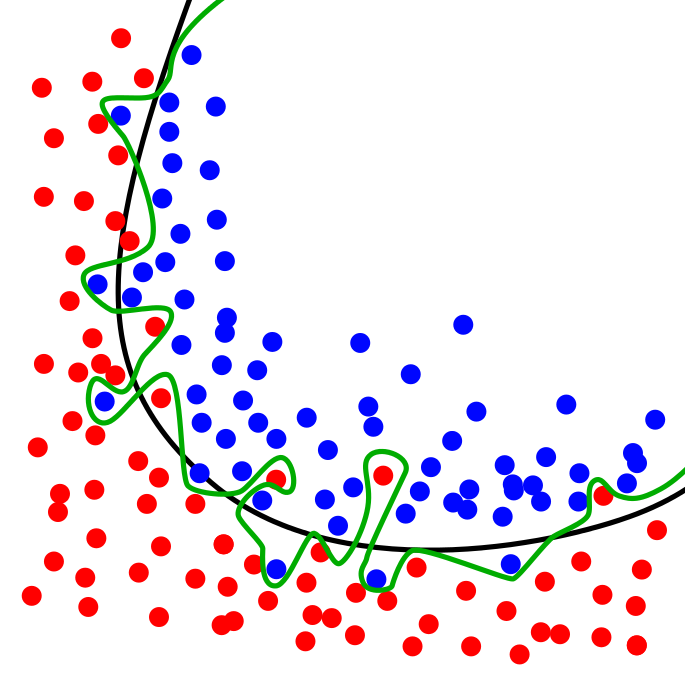
\includegraphics[scale=0.4]{imgs/overfitting}
  \caption{Modelo de aprendizado em um problema de duas classes, a linha preta indica uma função mais generalista, enquanto a linha verde representa uma função com acurácia maior em relação às amostras de treinamento, mas que provavelmente sofre de \textit{overfitting.}}
  \label{fig:overfitting}
\end{figure}

Para detectar problemas de \textit{overfitting}, pode-se testar o modelo em diversas outras bases de amostras, medindo a variância da acurácia entre estas bases. Uma alta variância indica que o modelo não é genérico o suficiente, apontando para um provável caso de \textit{overfitting}.

Um método bastante utilizado para medir a generalização de um modelo de aprendizado é a validação cruzada. O conceito principal deste método é o particionamento do conjunto de amostras em um número de subconjuntos mutuamente exclusivos, utilizando um dos subconjuntos como base de treinamento e as demais como bases de validação do modelo treinado.

A técnica de validação cruzada conhecida como \textit{k-fold} divide a base em $k$ subconjuntos de mesmo tamanho, escolhe um dos subconjuntos como base de treinamento e utiliza os demais subconjuntos como bases de testes deste primeiro subconjunto. O procedimento é repetido $k$ vezes, de forma que todos os subconjuntos possam ser utilizados para construir uma versão de modelo de aprendizado e ser validados pelos demais subconjuntos. A precisão do modelo é obtida pela equação \ref{eq:kfold}, onde $k$ é o número de subconjuntos e $y_i - y'_i$ é a diferença entre o valor esperado e o valor predito pelo modelo.

\begin{equation}
  \displaystyle Ac_f = \frac{1}{k} \sum_{i=1}^k{(y_i - y'_i)}
\label{eq:kfold}
\end{equation}

Uma outra avaliação importante a ser feita é a da relação entre a taxa de acerto (verdadeiros positivos) e  a taxa de falsos positivos. Para tal análise, pode ser feito o estudo da curva ROC (do inglês \textit{Receiver Operating Characteristic}), um gráfico bidimensional que exibe no eixo y o percentual de verdadeiros positivos na amostra e, no eixo x, o percentual de falsos positivos da mesma amostra (figura \ref{fig:roc}).

\begin{figure}[h]
  \centering
  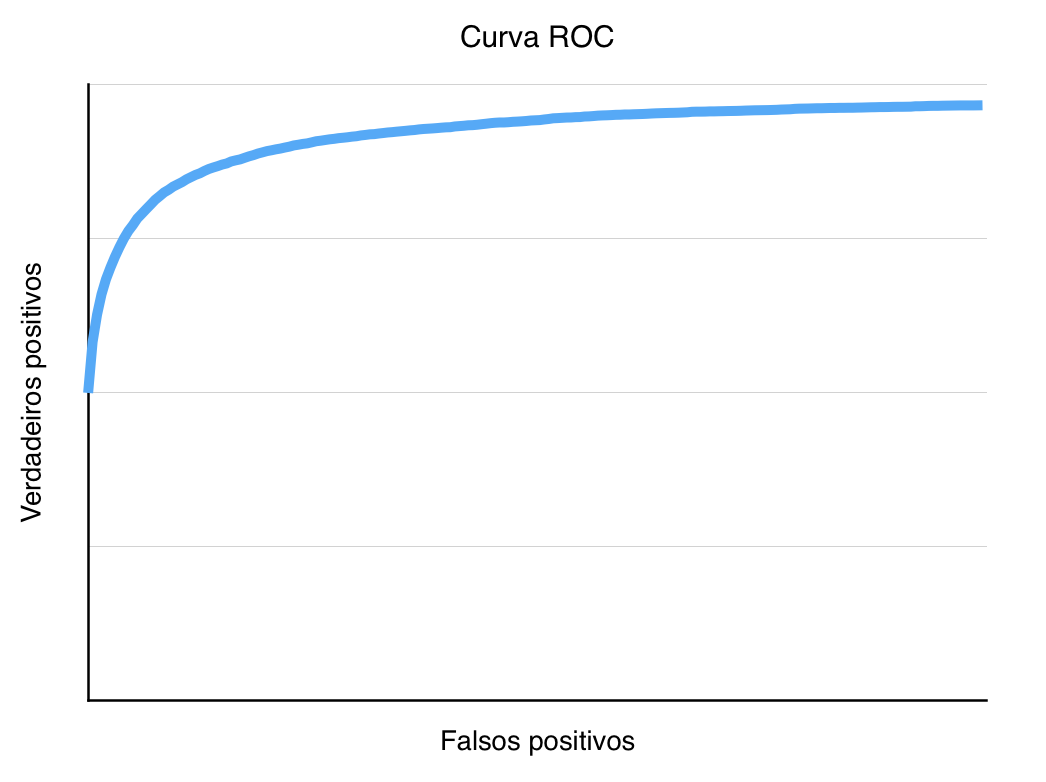
\includegraphics[scale=0.6]{imgs/roc}
  \caption{Exemplo de gráfico para análise de curva ROC}
  \label{fig:roc}
\end{figure}

Originalmente utilizada em detecção de sinais para mostrar a relação entre sensibilidade (taxa de acerto) e o inverso da especificidade (alarme falso) em canais com ruído, pode-se utilizar este gráfico na avaliação de modelos de aprendizagem de máquina. Em geral, o cálculo da área abaixo da linha do gráfico é calculado para determinar a relação entre verdadeiros positivos e falsos negativos para um conjunto de amostras. Quanto maior a área abaixo da curva, melhor é considerado o aprendizado sob esta avaliação.

Uma vez que a fundamentação teórica necessária foi coberta, é necessário fazer um levantamento na literatura pelos trabalhos considerados estado da arte em suas respectivas áreas. O capítulo a seguir trata deste levantamento.

\chapter{Trabalhos Relacionados}\label{cap:trabalhos}

A floresta amazônica é tema recorrente em diversas áreas de pesquisa, incluindo a área de sensoriamento remoto. Trabalhos vindos desta área costumam utilizar técnicas computacionais que pertencem ao estado da arte para analisar imagens que cobrem grandes áreas, sejam essas de espectro visível ou mesmo de RADAR ou LIDAR, e inferir as mais diversas informações sobre as regiões estudadas.

Trabalhos como os de \citeonline{almeidafilho:1998}, \citeonline{vasconcelos:2001}, \citeonline{lu:2012} e \citeonline{ferreira:2012} se utilizam de imagens com 6 bandas multiespectrais e 1 banda termal do satélite LANDSAT da região amazônica para determinar a cobertura de terreno das áreas inspecionadas. Estes trabalhos têm foco nos tipos de vegetação que cobrem o terreno, classes tais como floresta, capoeira, vegetação secundária, ou até mesmo espécies e grupos de plantas. Há trabalhos mais elaborados, como o de \citeonline{espiritosanto:2005}, que se utiliza das mesmas imagens do satélite LANDSAT, mas analisa amostras multitemporais, ou seja, imagens da mesma região em diversos sobrevoos do satélite, com o objetivo conseguir informações sobre mudanças na cobertura vegetal do terreno.

Há ainda trabalhos como o de \cite{azevedo:2014}, que utiliza como fonte de dados o satélite COSMO-SkyMed,  que disponibiliza imagens duais multitemporais da região amazônica. Estudos como o de \citeonline{latorre:2007} vão além e mesclam os dados de diversas fontes diferentes, utilizando técnicas de fusão de imagens.

Apesar dos resultados alcançados, os trabalhos sobre a classificação de imagens da floresta amazônica geralmente avaliam a cobertura vegetal da região, sem qualquer menção a elementos antrópicos, utilizando para isso imagens termais ou multiespectrais de diversos satélites. Dada a natureza relativamente lenta das mudanças de cobertura vegetal de terreno e o tamanho das áreas estudadas, é compreensível que satélites sejam utilizados.

Para o trabalho aqui apresentado, no entanto, os objetos de interesse mudam rapidamente, e a grande cobertura de área proporcionada por imagens de satélite deve dar lugar a imagens feitas por veículos aéreos, com maior proximidade e disponibilizadas com mais rapidez em uma missão real de patrulhamento ambiental. A base de imagens disponível para o trabalho é composta exclusivamente por imagens de espectro visível, por isso, muitas das técnicas e conclusões dos trabalhos citados acima não são prontamente transferíveis para este trabalho.

Os trabalhos relacionados apresentados nesta seção foram divididos primeiramente por assunto: de início, nos concentramos nos trabalhos publicados em segmentação de imagens que são considerados estado da arte, uma vez que esta é o primeiro desafio técnico a ser enfrentado pelo trabalho proposto. Depois, fazemos o levantamento de trabalhos relevantes sobre classificação de imagens aéreas. Em uma etapa posterior, investigamos trabalhos relacionados na área de detecção de anomalias.

As seções a seguir apresentam os trabalhos relacionados em ordem própria.  A seção \ref{sec:trSegmentacao} apresenta os trabalhos sobre segmentação de imagens de acordo com a ordem apresentada no trabalho de comparação realizado por \citeonline{arbelaez:2011}, explanado com mais detalhes em seguida. As seções \ref{sec:trClassificacao} e \ref{sec:trAnomalias} apresenta os trabalhos relacionados sobre classificação de imagens aéreas e detecção de anomalias, ambas em ordem cronológica de publicação.

Cada artigo é descrito com suas características, vantagens e desvantagens. No fim de cada seção, é apresentada uma tabela de comparação entre os trabalhos levantados.

\section{Segmentação de imagens}\label{sec:trSegmentacao}

Os trabalhos relacionados nesta seção foram escolhidos por terem obtido os maiores índices de precisão e revocação em uma base de dados de imagens naturais bastante conhecida pela comunidade de processamento de imagens, \textit{Berkeley Segmentation Data Set and Benchmarks 500}, também conhecida como BSDS500. Uma comparação entre os mais promissores algoritmos de segmentação de imagens foi realizada por \citeonline{arbelaez:2011}, consistindo na segmentação das imagens presentes no BSDS500 manualmente por seres humanos, e depois segmentadas pelos diversos algoritmos testados. A precisão e revocação de cada algoritmo são obtidas através de comparação com a segmentação manual.

Para reduzir ainda mais o número de algoritmos a serem inspecionados para este trabalho, a revisão de \citeonline{yuan2:2013} compara os mesmos algoritmos que \citeonline{arbelaez:2011} investigaram, mas dessa vez em uma base de imagens aéreas. A metodologia é a mesma usada no BSDS500, mas com uma base especializada. Os algoritmos com os melhores resultados foram selecionados para serem utilizados na construção deste trabalho de pesquisa, e coincidem com os resultados do trabalho de \citeonline{arbelaez:2011}. Os seis algoritmos selecionados serão discutidos a seguir.

O trabalho de \citeonline{deng:2001} trata de um algoritmo chamado JSEG, que obtém a segmentação da imagem em duas etapas. A primeira é a  quantização das cores da imagem em diversas classes. Baseada nessas cores quantizadas, a segunda etapa computa o valor de uma variável \textit{J} indicando a intensidade das bordas e utiliza um método de crescimento de região para segmentar a imagem com base no valor \textit{J}. O algoritmo ainda permite que o utilizador especifique o tamanho da janela para computar o valor de \textit{J}, o que torna o método bastante flexível para imagens de naturezas diferentes. Em imagens aéreas de escala considerável, como as utilizadas neste trabalho, pode-se usar uma janela diminuta, já que os detalhes importantes podem ser bem pequenos. Para diminuir super-segmentação, os segmentos encontrados na segunda etapa são fundidos de acordo com seus histogramas coloridos.

A abordagem utilizando mean-shift desenvolvida por \citeonline{comaniciu:2002} oferece uma ferramenta interessante para resolver o problema de segmentação de imagens. O algoritmo computa vetores de mean-shift iterativamente para mapear pixels para o domínio espacial e de cores do centro de seus agrupamentos (\textit{clusters}). Após a convergência, os \textit{clusters} são fundidos de acordo com parâmetros de similaridade. Parâmetros como largura de banda espacial, de cores e o tamanho do menor \textit{cluster} podem ser utilizados para adequar o algoritmo ao problema em questão.

O algoritmo \textit{Multi-resolution Region Merging Segmentation} (MSEG), descrito por \citeonline{felzenszwalb:2004}, é amplamente usado pela comunidade de sensoriamento remoto. No MSEG, o aumento na heterogeneidade no momento da junção de um par de segmentos é computado como uma soma ponderada de medidas de coloração e morfologia. O procedimento de junção é realizado iterativamente, e  junta os pares de segmento que resultam no menor aumento de heterogeneidade possível, até que a soma exceda um limiar, que pode ser parametrizado pelo utilizador. Sob a óptica de grafos, os pixels são tratados como nodos e os pesos de suas arestas representam a diferença entre características entre os pixels. Um segmento corresponde a um componente conectado nesse grafo. Um parâmetro é utilizado para definir a escala observada na segmentação, o que influi no tamanho e no número dos segmentos resultantes.

O algoritmo de \textit{Statistical Region Merging} (SRM) publicado por \citeonline{nock:2004} utiliza um procedimento simples de junção acompanhado por uma operação de ordenação para segmentar imagens com eficiência. Duas regiões são unidas se os valores médios dos pixels das duas regiões estão mais próximos que um limiar previamente definido. A coesão da segmentação pode ser controlada por um parâmetro definido pelo usuário.

O trabalho de \citeonline{yuan:2013} apresenta um algoritmo chamado \textit{Factorisation-based segmentation} (FSEG). O FSEG primeiramente computa o histograma espectral para cada pixel da imagem, que é um amalgama de diversas respostas aos filtros em uma janela local. Esse algoritmo é baseado na proposta de que cada característica pode ser aproximada por uma combinação linear de diversas características representativas e suas combinações ponderadas. Por fim, um pixel é dito pertencente à região com maior peso. O algoritmo FSEG utiliza decomposição de valores singulares e fatoração de matrizes não-negativas para aumentar a eficiência computacional da segmentação, o que é atrativo quando o tempo de processamento é um fator importante.

O algoritmo gPb-owt-ucm introduzido por \citeonline{arbelaez:2011} realiza segmentação em várias etapas. Primeiramente a técnica combina informações de intensidade, textura e coloração para computar vetores que servirão como  detectores de contorno. Posteriormente, uma técnica de \textit{watershed} é aplicada à saída do detector de contornos para produzir uma segmentação hierárquica da imagem. Uma vantagem importante desta técnica é a possibilidade de ajustar a escala de segmentação, portanto o usuário pode escolher uma escala que mais se adequa ao tipo de imagem do problema, evitando segmentação excessiva da imagem.

A tabela \ref{tab:sumarioSegmentacao} exibe os resultados encontrados por \citeonline{yuan2:2013}, juntamente com uma descrição das características das diversas técnicas de segmentação de imagens levantadas neste trabalho.

\begin{table}[h]
\ABNTEXfontereduzida
\centering
\begin{tabulary}{\linewidth}{|L|L|C|C|}
\hline
\textbf{Técnica} & \textbf{Características} & \textbf{Prec. bordas} & \textbf{Prec. regiões } \\ \hline
Manual      & Não aplicável    & 69\% & 84\% \\ \hline
gPb-owt-ucm & Cor, borda       & 65\% & 69\% \\ \hline
FSEG        & Textura          & 61\% & 66\% \\ \hline
SRM         & Cor, intensidade & 60\% & 60\% \\ \hline
JSEG        & Cor, borda       & 56\% & 66\% \\ \hline
MSEG        & Cor, morfologia  & 57\% & 50\% \\ \hline
Mean-shift  & Cor, posição     & 58\% & 48\% \\ \hline
\end{tabulary}
\caption{Comparação entre as técnicas de segmentação de imagens, ordenados por desempenho decrescente, conforme resultados em \citeonline{yuan2:2013} }
\label{tab:sumarioSegmentacao}
\end{table}

Tanto na revisão feita por \citeonline{arbelaez:2011} com a base de imagens naturais BSD500, quanto na comparação feita por \citeonline{yuan2:2013} em uma base de imagens aéreas, o algoritmo gPb-owt-ucm de \citeonline{arbelaez:2011} possui um desempenho superior aos demais algoritmos avaliados. Nenhum dos trabalhos faz qualquer avaliação sobre o custo computacional dos algoritmos, nem sobre o tempo de execução durante os experimentos.

Conforme descrito em detalhes no capítulo \ref{cap:metodologia}, a abordagem escolhida neste trabalho para encontrar elementos antrópicos em imagens aéreas da floresta amazônica passa pela classificação das regiões de imagens produzidas por um algoritmo de segmentação. Por este motivo, um levantamento bibliográfico também foi feito sobre classificação de imagens aéreas.

\section{Classificação de imagens aéreas}\label{sec:trClassificacao}

Os trabalhos relacionados sobre classificação de imagens aéreas foram selecionados de acordo com suas semelhanças com o trabalho proposto neste documento. Todos tratam de imagens aéreas ortogonais, ou seja, com inclinação de aproximadamente 90\degree em relação ao solo, em cenas naturais e com bases de dados com forte presença de vegetação. Os trabalhos relacionados expressam diferentes formas de classificação das imagens: classificação de pixels individuais, blocos, segmentos ou superpixels.

É importante também destacar que todos os trabalhos descritos a seguir possuem imagens em escala similar às imagens de VANTs, baseando-se na altitude regular de operação desses equipamentos. O fato de terem sido coletadas com VANTs ou não, é de pouca importância para efeitos de comparação, já que os aspectos técnicos das imagens são similares.

O trabalho de \citeonline{dubuisson:2000} apresenta uma técnica de segmentação focada em imagens aéreas coloridas que realiza segmentações separadamente por cor e textura, para no final unir as duas e chegar a uma segmentação final utilizando um algoritmo de classificação por máxima verossimilhança (\textit{Maximum Likelihood}). Os autores chegara à conclusão que informações de cor são mais eficientes para a localização de bordas, enquanto a textura provê uma classificação menos ruidosa das regiões da imagem. A computação isolada das características foi importante para entender melhor que tipos de atributos contribuem melhor em que etapas do trabalho, mas a metodologia utilizada para mesclar as segmentações é pouco explicada no artigo. O objetivo do trabalho de \citeonline{dubuisson:2000} é a atualização de mapas antigos a partir de imagens recentes, mas pode facilmente ser utilizado na classificação de cobertura de terreno, ou de regiões previamente segmentadas.

De acordo com \citeonline{sadgal:2005}, o processamento de imagens digitais que representam cenas naturais requer elaboração substancial em todos os níveis: pré-processamento, segmentação, reconhecimento e interpretação. O trabalho apresentado sugere uma abordagem onde todas essas etapas acontecem em um único nível, e propõe um modelo de visão que tenta generalizar o reconhecimento de objetos utilizando categorização e cooperação.  A solução proposta combina processos estocásticos, dentre os quais Inferência Bayesiana, Campos Aleatórios de Markov, com métodos não-estocásticos como Redes Neurais Artificiais. Esta diversidade de métodos é utilizada na segmentação e na extração de características de cores, texturas e formas, que depois são usadas na classificação dos objetos. Uma vantagem importante deste método é a possibilidade de paralelizar o processo de classificação, uma vez que as diversas técnicas são fundidas no final do processo, ao invés de serem aplicadas em cascata. Embora os resultados pareçam ser satisfatórios em imagens naturais, pouco é dito sobre como o processo de fusão de classificadores é feito, e nenhuma implementação ou base de imagens está disponível publicamente.

A pesquisa realizada por \citeonline{ahmadi:2013} tem como objetivo fazer segmentação e classificação de imagens aéreas, pixel a pixel. Para tal, diversos classificadores e atributos das imagens são testados, chegando-se a conclusão de que o uso do algoritmo de KNN em características de cor e textura, mais precisamente o filtro de Gabor \cite{fogel:1989} dos canais de matiz, saturação e intensidade (HSV) de cada pixel, obtiveram os melhores resultados dentre os algoritmos testados. Este trabalho argumenta que métodos estabelecidos na literatura costumam classificar as imagens com base em segmentos, o que supostamente costuma levar mais tempo que uma abordagem que classifique diretamente os pixels, mas os resultados do experimentos não são particularmente precisos, com acurácia máxima de 82,23\% na base de imagens testada.

A dissertação de mestrado de \citeonline{fernandes:2008} descreve uma solução de detecção de áreas de desmatamento em imagens de radar e satélite da região amazônica. Para tanto, uma segmentação das imagens utilizando a técnica de \textit{meanshift} é realizada, cabendo ao algoritmo de aprendizado SVM a classificação destes segmentos em "área desmatada" ou "área não-desmatada". Com a precisão média geral de 87\% de acurácia para imagens de satélite e 74\% para imagens de radar, a autora considera que os resultados foram satisfatórios, visto que apenas 2,3\% dos segmentos analisados apresentam erros graves para a classe de interesse. A mesma métrica gira em torno de 5,8\% para as imagens de radar. Este é o único trabalho relacionado que se utilizou de imagens de satélite, mas foi incorporado à bibliografia por se tratar de imagens da região amazônica e com vários objetivos em comum.

O trabalho de \citeonline{ghiasi:2013} realiza segmentação e classificação de tipos de terreno em imagens aéreas através de dois passos: primeiramente a imagem é dividida em superpixels, utilizando a técnica de fluxos geométricos de \citeonline{levinshtein:2009}; posteriormente, cada superpixel tem suas características de textura e cor extraídas e é classificado através do algoritmo KNN. As características apontadas como mais úteis pelos autores são o Local Binary Pattern Histogram Fourier (LBP-HF) \cite{ahonen:2009} para informações de textura e histograma dos canais RGB para informações sobre cores. Os autores do artigo alegam realizar o processo em tempo real, com precisão superior a 95\% em todas as classes utilizadas. Apesar do cenário e região apresentados pelo trabalho de \citeonline{ghiasi:2013} serem diversos dos nossos, o tipo de imagem, as condições de aquisição e a diferenciação de elementos antrópicos (edificações, neste caso) estabelecem uma forte relação entre os dois trabalhos.

A tabela \ref{tab:sumarioClassificacao} apresenta um sumário dos trabalhos levantados nesta seção, ordenados conforme aparição.

\begin{table}[h]
\ABNTEXfontereduzida
\centering
\begin{tabulary}{\linewidth}{|L|L|L|L|C|}
\hline
\textbf{Trabalho} &  \textbf{Aprendizado} & \textbf{Amostra} & \textbf{Problema investigado} &  \textbf{Precisão} \\ \hline
Dub-Jolly & Máxima verossimilhança & Pixel      & Atualização de mapas           & 91,86\% \\ \hline
Sadgal    & Redes neurais          & Blocos     & Classificação de terreno       & -       \\ \hline
Ahmadi    & KNN                    & Pixel      & Classificação de terreno       & 82,23\% \\ \hline
Fernandes & SVM                    & Segmentos  & Detecção de áreas desmatadas   & 87\%    \\ \hline
Ghiasi    & KNN                    & Superpixel & Busca por objetos de interesse & 95\%    \\ \hline
\end{tabulary}
\caption{Comparação entre os trabalhos sobre classificação de imagens aéreas}
\label{tab:sumarioClassificacao}
\end{table}

Os trabalhos relacionados à classificação de imagens aéreas exploram pouco a problemática de detecção de anomalias. O trabalho aqui apresentado tem como objetivo final a classificação e detecção de regiões anômalas à paisagem natural, portanto definidas como antrópicas. Tais regiões em um ambiente natural vasto como o da floresta amazônica, tendem a ter ocorrência muito baixa, portanto podem ser consideradas anomalias.

Com a preocupação de que modelos de aprendizado supervisionados convencionais tenham dificuldade em reconhecer classes tão pouco representadas em uma base de treinamento, um levantamento foi feito por trabalhos na área de detecção de anomalias utilizando aprendizagem de máquina.

\section{Detecção de anomalias}\label{sec:trAnomalias}


\todo[inline]{Não há trabalhos que busquem detectar anomalias? Como você estuda a detecção de anomalias, eu creio que você precisa descrever trabalhos que investiguem esse tópico, mesmo que não envolvam imagens. Por exemplo, o trabalho de Hadjadji, Chibani e Guerbai (2014) precisa ser descrito aqui, assim como outros trabalhos nessa linha. Esses trabalhos são importantes para justificar a escolha dos quatro cenários que você investigou no seu trabalho.}

\todo[inline]{
	Trabalho
		caracteristicas
		vantagens
		desvantagens
		relação com meu trabalho
	Tabela comparativa
}

O trabalho de \citeonline{pla:2013} consiste em um breve resumo do estado da arte de classificação unária para reconhecimento de imagens, seguido de uma aplicação real de classificação de pixels. Os autores apresentam os resultados da detecção de vegetação (classe majoritária) \textit{versus} solo nu (classe minoritária) em uma base de imagens hiperespectrais de satélite com 207 bandas, formado da fusão de diversas fontes. Com 100\% de verdadeiros positivos e 9\% de falsos positivos para a classe majoritário, o trabalho não dá detalhes sobre a distribuição das classes na base de dados nem apresenta resultados para a classe minoritária, portanto, não é possível saber se os resultados são satisfatórios. A utilidade e relação do trabalho de \citeonline{pla:2013} com este aqui apresentado residem no uso do algoritmo One-class Support Vector Machines (OC-SVM), considerado estado da arte em diversas aplicações de aprendizado unário e na temática do problema apresentado, que se utiliza de imagens aéreas de regiões com intensa cobertura vegetal.

\todo[inline]{falar sobre a tabela de resultados}

\begin{table}[h]
\ABNTEXfontereduzida
\centering
\begin{tabulary}{\linewidth}{|L|L|L|L|C|}
\hline
\textbf{Trabalho} &  \textbf{Algoritmo} & \textbf{Amostra} & \textbf{Problema investigado} &  \textbf{Precisão} \\ \hline
Pla (2013) & OC-SVM & Pixel & Detecção de vegetação & 91,86\% \\ \hline
\end{tabulary}
\caption{Comparação entre os trabalhos sobre detecção de anomalias}
\label{tab:sumarioAnomalias}
\end{table}

Este trabalho pretende adaptar ou enriquecer os métodos utilizados na literatura, aplicando-os especificamente à detecção de elementos antrópicos em imagens aéreas da floresta amazônica, que possui seus desafios característicos, visto que o tipo de terreno e vegetação apresentam padrões diferentes dos vários trabalhos realizados em áreas urbanas ou florestas temperadas. Os trabalhos encontrados relacionados à floresta amazônica comumente se utilizam de outros tipos de sensores como RADAR e LIDAR, além de câmera de espectro visível, como pode ser visto nos trabalhos de \citeonline{linhares:2014} e \citeonline{santos:2005} e \citeonline{fernandes:2008}. Estes trabalhos também tendem a se preocupar com dados temporais, como avanço do desmatamento e levantamento de grandes áreas.

O diferencial deste trabalho está na aplicação ao tema de vigilância ambiental através de VANTs e a preocupação com disponibilização dos conjuntos de dados rotulados para trabalhos futuros na mesma problemática. Mais detalhes sobre o método proposto serão discutidos no capítulo \ref{cap:metodologia}.

\chapter{Metodologia}\label{cap:metodologia}

Neste capítulo é descrita a sequência de etapas que serão realizadas neste trabalho para que os objetivos de pesquisa sejam alcançados.

Em imagens aéreas como as utilizadas neste trabalho, é comum que os elementos que indicam presença humana sejam relativamente grandes (pista de pouso, estradas, clareiras, etc.), podendo ser definidas como uma região durante a segmentação da imagem.

Classificar pixels tende a ser custoso, visto que mesmo uma pequena imagem provê dezenas de milhares deles, que devem ter suas características extraídas e providas ao modelo de aprendizado, para que possam ser classificados. Portanto, utilizar técnicas de segmentação de imagem para agrupar os pixels espacialmente e caracteristicamente relacionados em uma única amostra não só possibilita uma execução mais rápida da solução computacional, como também torna o resultado final menos ruidoso.

Por este motivo, a arquitetura para a solução proposta prevê uma etapa de segmentação das imagens, seguida de uma etapa de classificação, responsável pela determinação do tipo de cada região encontrada na segmentação. Desta forma, elementos antrópicos podem ser separados como mais uma das regiões das imagens e classificados como tal. O diagrama da arquitetura geral da solução pode ser visto na figura \ref{fig:metDiagramaGeral}.

\begin{figure}[h]
    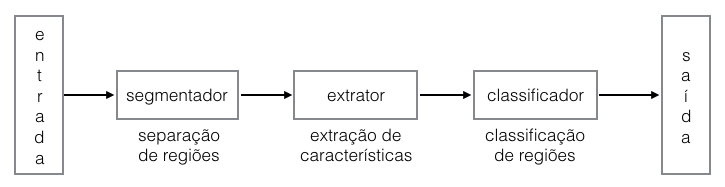
\includegraphics[width=\textwidth]{imgs/arquitetura_geral}
    \caption{Arquitetura geral da solução a ser desenvolvida para detecção de elementos antrópicos em imagens aéreas da floresta amazônica}
    \label{fig:metDiagramaGeral}
\end{figure}

A ideia geral é que imagens aéreas de regiões florestais da Amazônia legal sirvam de entrada para o problema. Estas mesmas imagens serão particionadas em regiões por um segmentador. Em seguida, um extrator será utilizado para criar o vetor de características de cada segmento provido pela etapa anterior. Por fim, um classificador composto por um ou mais algoritmos de classificação será utilizado para rotular as regiões, com a finalidade de encontrar as regiões de elementos antrópicos. A saída do sistema pode, então, ser composta pelas regiões segmentadas e suas classificações finais.

Embora esta seja uma arquitetura simples, bastante difundida na literatura, nuances para o problema apresentado neste trabalho devem ser levadas em conta. Para chegarmos à conclusão de quais segmentadores, extratores e classificadores devem ser utilizados, são necessárias várias etapas de experimentação, validação e análise de resultados.

\section{Entrada}

Uma base de dados com imagens aéreas de floresta tropical precisa ser formada. Todas as imagens precisam ter as mesmas dimensões, condições visuais semelhantes e preferencialmente pertencerem à região de floresta amazônica, excluindo imagens de cidades e povoados da região.

Como serão processadas por uma etapa de segmentação, as imagens não sofrerão nenhum tipo de filtragem, ficando estas a cargo dos segmentadores a serem avaliados. A base de imagens gerada nesta etapa é um dos objetivos específicos deste trabalho.

\section{Segmentador}\label{sec:metSegmentador}

Para encontrarmos o segmentador ideal, os métodos de segmentação de imagens considerados estado-da-arte serão aplicados à uma parte da base de imagens aéreas da floresta amazônica. Conforme levantado no capítulo \ref{cap:trabalhos}, os seguintes métodos serão avaliados: Mean-shift, JSEG, MSEG, SRM, FSEG e gPb-owt-ucm. Estes métodos foram escolhidos por terem os melhores desempenhos em dois trabalhos comparativos de segmentação: o \textit{benchmark} de segmentação da base de imagens naturais BSD500, de \citeonline{arbelaez:2011}, e o \textit{benchmark} de segmentação de uma base de imagens aéreas de \citeonline{yuan2:2013}.

Também será realizado um experimento que funde as etapas de segmentação e classificação em uma só, utilizando algoritmos de aprendizado de máquina supervisionados para segmentar as imagens diretamente para suas classes (floresta, água, etc) pixel a pixel. Isto é importante para determinar se há ganhos reais na separação entre segmentação e classificação das imagens, ou se realizar todo o procedimento em um único passo produz melhores resultados de acurácia e custo computacional.

A base de dados também precisa ser segmentada manualmente por seres humanos, pois este será o \textit{ground-truth} usado para aferir o desempenho dos algoritmos de segmentação avaliados. Ainda é preciso aferir a consistência da segmentação manual realizada por seres humanos. Métricas de erros de consistência como o \textit{Local Consistency Error} (LCE) e \textit{Global Consistency Error} (GCE), descritos na seção \ref{sec:avaliacaopdi}, devem ser aplicados para a medição de desempenho de todos os algoritmos, bem como para validação da consistência interna da segmentação manual.

Esta etapa deve determinar o método de segmentação com melhores resultados, a ser utilizado na solução descrita pelo trabalho. A precisão e o tempo de execução devem ser utilizados para a avaliação do desempenho dos algoritmos testados. Em seguida, é preciso extrair as características dos segmentos gerados.

\section{Extrator}\label{sec:metExtrator}

Os algoritmos de classificação lidam com variáveis numéricas inteiras, de ponto flutuante e em alguns casos, dados textuais. No entanto, para classificar imagens, ou no caso deste trabalho, segmentos de imagens, é preciso que um conjunto de características seja extraído dos pixels destas imagens ou regiões e disponibilizados para o modelo de classificação.

Nesta etapa serão testadas diversas características disponíveis na literatura de processamento digital de imagens, especialmente informações sobre cor, intensidade, textura e morfologia destas amostras. A escolha das características foi baseada, inicialmente, nas características utilizadas em trabalhos relacionados de classificação de imagens aéreas: canais RGB para descrição de cores, histogramas de intensidade, \textit{Local Binary Patterns} para descrição de texturas e transformada de Hough para detecção e descrição de formas geométricas, em especial linhas retas.

Os atributos também deverão passar por um processo de seleção baseada em correlação, o CFS. O objetivo é diminuir a dimensionalidade do vetor de características e avaliar se há ganho no desempenho e generalização dos algoritmos de aprendizado, utilizando este subconjunto do vetor de características original.

Como requisito da composição da base de dados de segmentos, bem como para avaliação e otimização do vetor de características, todas as amostras geradas pela etapa de segmentação devem ser rotuladas manualmente e contar com a avaliação de especialistas na inspeção deste tipo de imagem. Com a base devidamente criada e rotulada, experimentos para determinar os classificadores mais adequados podem ser feitos.

\section{Classificador}\label{sec:metClassificador}

Nesta etapa, quatro estratégias de classificação presentes na literatura serão abordadas: classificadores multi-classe, binários, unários e conjuntos de classificadores unários. Elas não demandam alterações na arquitetura geral da solução, mas mudam a forma como a base é rotulada e organizada. As métricas de avaliação do aprendizado precisam ser ponderadas para cada estratégia.

É importante destacar que a classe de interesse, elementos antrópicos, permanece a mesma em todas as abordagens, e sua inspeção mais cuidadosa é vital na avaliação de todos os métodos utilizados.

\subsection{Classificador multi-classe}

Nesta estratégia, a base de segmentos gerada será rotulada entre cinco classes possíveis: floresta, vegetação rasteira, água, terra e elemento antrópico. Diversos algoritmos que possibilitam clasificação multi-classe serão utilizados, tendo em mente que é importante testar métodos simbólicos, bayesianos, não-paramétricos, máquina de vetores de suporte, entre outros.

Todos os métodos devem ser testados com a base completa de segmentos, mas também com a base pré-processada por um seletor de características, que será responsável pela redução do vetor de características do problema. Este detalhe do experimento servirá para determinar se a seleção de atributos nesta abordagem reduz a complexidade dos modelos gerados e o ruído na base de dados, possibilitando melhor taxa de aprendizagem.

Cada algoritmo deve ser responsável pela classificação de toda a base. Ao fim, métricas de aprendizado como acurácia, precisão e revocação serão utilizadas para comparar os métodos entre si.

\subsection{Classificador binário}

Neste cenário, a base de segmentos gerada será rotulada entre duas classes: elementos naturais e elementos antrópicos. A classe de elementos naturais agrupa o que originalmente seriam as classes de floresta, vegetação rasteira, água e terra.

Os classificadores utilizados serão os mesmos do experimento com classificadores multi-classe, visto que não há grande diferença metodológica nas duas abordagens. Todos os métodos também serão testados com seletores de características, e o impacto desta seleção também será avaliado.

Ao fim do experimento, as métricas propostas para o problema de aprendizado serão colhidas para cada método testado e utilizados para comparar os métodos entre si, bem como o impacto geral da seleção de atributos para esta abordagem.

\subsection{Classificador unário}

Assim como no experimento de classificadores binários, a base de dados de segmentos será dividida entre elementos naturais e elementos antrópicos, utilizando os mesmos critérios. À primeira vista, esta estratégia de aprendizado parece muito similar aos classificadores binários, mas a diferença está inicialmente nos algoritmos utilizados.

Como o aprendizado unário utiliza o conceito de classe majoritária e classe anômala (\textit{outlier}), é preciso definir que classes do problema exercerão estes papéis. Por uma simples questão de frequência estatística, fica definido que a classe de elementos naturais é a classe majoritária, enquanto a classe de elementos antrópicos é considerada a classe anômala.

Aqui também deve ser avaliado o impacto de um seletor de atributos aplicado ao vetor de características da base de dados, a fim de entender se há mudança significativa na taxa de aprendizado da classe anômala.

\subsection{Conjunto de classificadores unários}

Esta abordagem consiste na criação de modelos de aprendizado unários para cada classe do problema, exceto para a classe anômala. Sendo assim, um ou mais classificadores unários serão treinados para cada uma das classes de floresta, vegetação rasteira, água e terra.

A preparação da base de dados é um importante passo nesta estratégia de aprendizado, visto que diversas versões da base de segmentos terão de ser geradas, cada uma representando a classe não-anômala em questão como a classe majoritária e todas as demais como outliers.

O conjunto de classificadores criados serão agrupados em um \textit{ensemble} de classificadores e cada um dos modelos será utilizado na composição do veredito final, para a classificação da amostra. Diversas combinações de modelos e algoritmos deverão ser testadas, bem como diversas formas de combinar os resultados dos classificadores individuais.

Assim como todas as outras estratégias de classificação presentes neste trabalho, as métricas mais relevantes serão a acurácia, precisão e revocação da classe de interesse, de elementos antrópicos, que aqui é a classe anômala. As abordagens de classificação com melhor desempenho nestes quesitos ou mais promissoras devem ser apontadas ao fim destes experimentos.

\section{Saída}

 Os resultados dos experimentos anteriores devem sustentar a conclusão sobre quais métodos de segmentação e classificação são mais indicados para a solução. A saída da solução deve indicar quais segmentos da coleção de imagens original possuem elementos antrópicos. A avaliação do desempenho na detecção destes elementos é a métrica definitiva da adequação da solução para o problema proposto.

O próximo capítulo descreve os experimentos realizados e discute os resultados encontrados.

\chapter{Experimentos e Resultados Preliminares}\label{cap:experimentos}

\section{Base de dados}

A base de dados (imagens) utilizada advém do projeto GEOMA \cite{geoma}, financiado pelo Instituto de Pesquisas Espaciais (INPE). Trata-se de imagens coloridas, codificadas em JPEG e com 640 pixels de largura por 480 pixels de altura. A base é composta por fotografias ortogonais ao relevo (como pode ser visto na figura \ref{fig:amostra}), de altitudes variadas e tiradas a partir de aeronaves tripuladas, durante o trajeto entre diversas cidades da região amazônica.

No momento do início dos experimentos deste trabalho, estas imagens tiradas de aviões tripulados eram as únicas disponíveis publicamente. Podemos considerá-las válidas por terem sido tiradas em altitude de vôo compatível com as missões de VANTs de vigilância, entre 900 e 1.100 metros do solo. Como este trabalho tem como objetivo utilizar apenas câmeras de espectro visível, são dispensáveis comparações de sensores com VANTs que eventualmente possuam sonar, câmeras infravermelho ou outros tipos de sensores.

\begin{figure}[h]
  \centering
  \begin{subfigure}[b]{0.3\textwidth}
    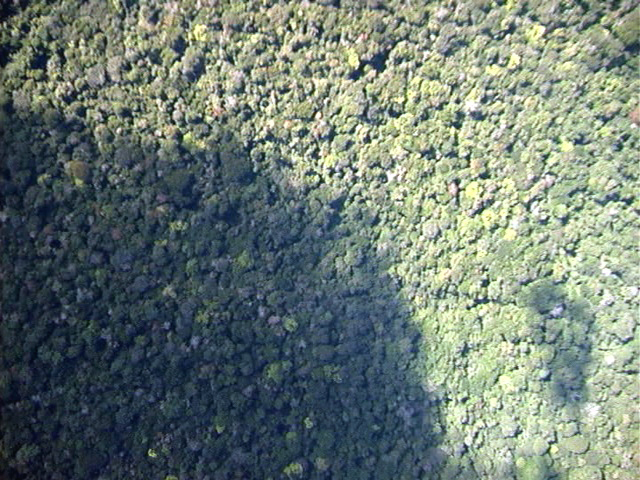
\includegraphics[width=\textwidth]{imgs/amostra1}
  \end{subfigure}%
  ~
  \begin{subfigure}[b]{0.3\textwidth}
    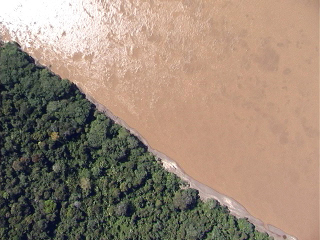
\includegraphics[width=\textwidth]{imgs/amostra2}
  \end{subfigure}%
  ~
  \begin{subfigure}[b]{0.3\textwidth}
    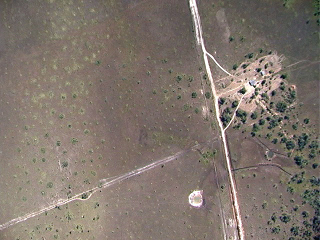
\includegraphics[width=\textwidth]{imgs/amostra3}
  \end{subfigure}%
  \caption{Amostras da base de dados}
  \label{fig:amostra}
\end{figure}

A base possui um total de 3.044 imagens, com dimensão total de 1,02 Gigabytes de dados. Cerca de 150 imagens foram utilizadas nos experimentos até o momento, visto que um grande esforço precisa ser despendido na classificação manual das imagens em todas as etapas do experimento, consumindo um tempo considerável.

Para facilitar a classificação manual foi construída uma ferramenta gráfica que permite ao usuário segmentar e classificar as regiões das imagens de acordo com as classes disponíveis (figura \ref{fig:visualClassifier}). A saída deste aplicativo é uma coleção, para cada imagem, de informações sobre bordas das regiões e a classificação de cada pixel. Posteriormente essas informações serão confrontadas com o resultado da segmentação e primeiro nível de classificação da solução.

\begin{figure}[h]
  \centering
  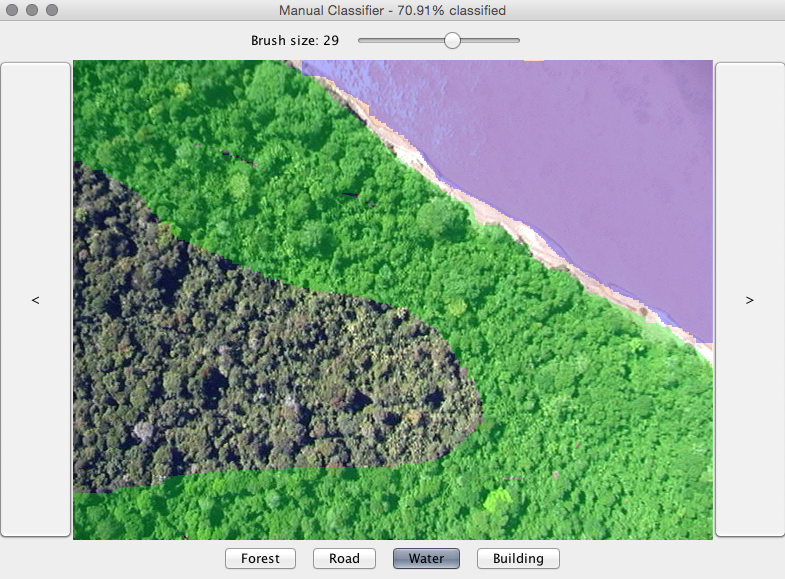
\includegraphics[width=0.7\textwidth]{imgs/visualClassifier}
  \caption{Ferramenta para segmentação e classificação manual das imagens em regiões}
  \label{fig:visualClassifier}
\end{figure}

\section{Segmentação}

Para determinar qual dos algoritmos de segmentação levantados na pesquisa bibliográfica teria melhor desempenho na base de dados utilizada neste trabalho, todos foram implementados ou adaptados. Os algoritmos foram testados no conjunto inicial de 150 imagens e comparados com a segmentação manual realizada nas mesmas imagens.

Para avaliar as diferentes segmentações, o método introduzido por \citeonline{martin:2001} foi utilizado. Este método consiste na sobreposição de regiões e comparação de informações sobre localização e orientação dos elementos de borda (\textit{edgels}).

Os resultados do experimento são apresentados na tabela \ref{tab:experimentoSegmentacao}:

\begin{table}[h]
\ABNTEXfontereduzida
\centering
\begin{tabulary}{\linewidth}{|L|R|R|}
\hline
\textbf{Algoritmo} & \textbf{Precisão} & \textbf{Tempo/imagem} \\ \hline
Mean-shift  & 97,2\% & 6,39 s \\ \hline
JSEG        & 96,3\% & 14,82 s \\ \hline
MSEG        & 94,1\% & 0,33 s \\ \hline
SRM         & 91,9\% & 4,66 s \\ \hline
FSEG        & 81,4\% & 13,91 s \\ \hline
gPb-owt-ucm & 72,2\% & 237,32 s \\ \hline
\end{tabulary}
\caption{Comparação de métodos de segmentação em parte da base de imagens deste trabalho, ordenados por precisão}
\label{tab:experimentoSegmentacao}
\end{table}

O algoritmo Mean-shift, além de ter conseguido a melhor precisão na nossa base de dados, conseguiu um bom desempenho de tempo. Com isso, pudemos determinar que ele será o algoritmo utilizado no trabalho, para a segmentação inicial das imagens.

O método JSEG conseguiu uma precisão bastante próxima do Mean-shift e será considerado uma alternativa, embora o tempo de segmentação deste algoritmo seja consideravelmente maior. A imagem \ref{fig:comparacaoSegmentacao} mostra a saída de alguns dos métodos testados, para fins de comparação visual.

\begin{figure}[htb]
	\centering
	\begin{minipage}[l]{0.51\linewidth}
		\begin{subfigure}[b]{\linewidth}
			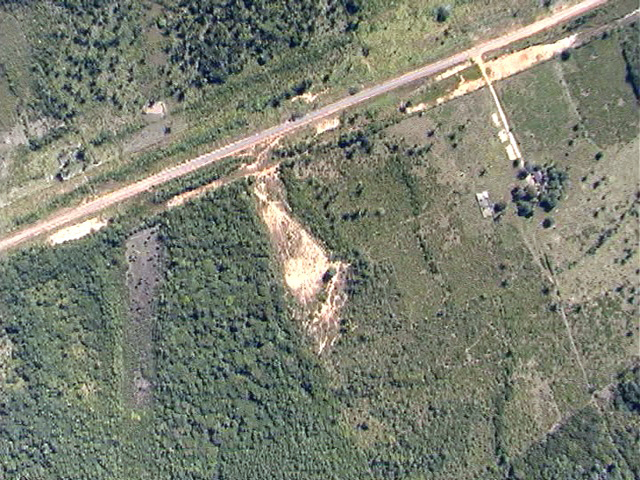
\includegraphics[width=\linewidth]{imgs/seg_original}
			\caption{Imagem original}
		\end{subfigure}%
	\end{minipage}
	\begin{minipage}[r]{0.48\linewidth}
		\begin{subfigure}{.47\linewidth}
			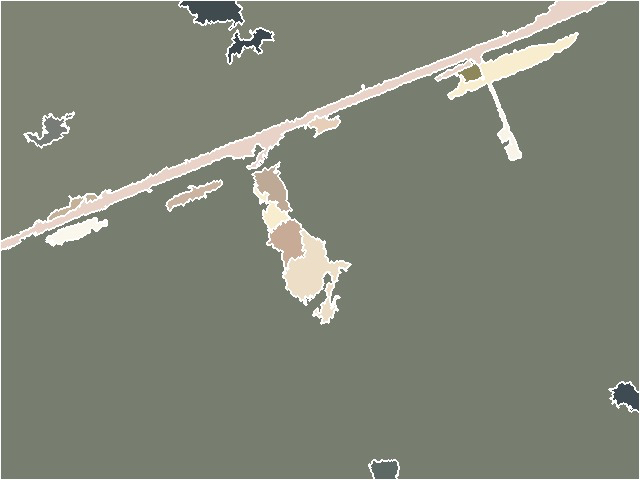
\includegraphics[width=\linewidth]{imgs/seg_meanshift}
			\caption{Mean-shift}
		\end{subfigure}
		\begin{subfigure}{.47\linewidth}
			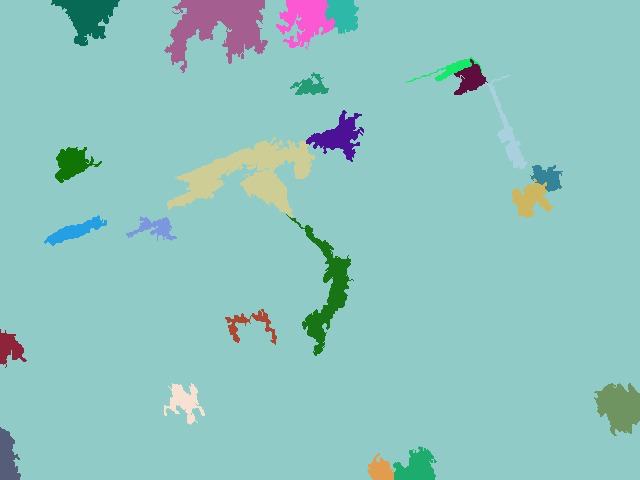
\includegraphics[width=\linewidth]{imgs/seg_mseg}
			\caption{MSEG}
		\end{subfigure}%
		\\
		\begin{subfigure}{.47\linewidth}
			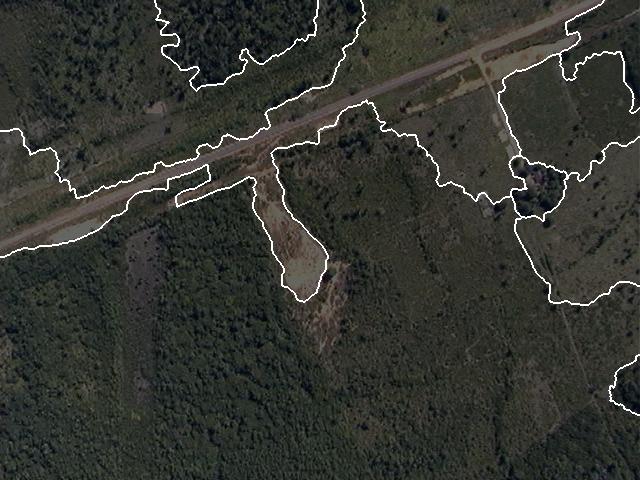
\includegraphics[width=\linewidth]{imgs/seg_jseg}
			\caption{JSEG}
		\end{subfigure}
		\begin{subfigure}{.47\linewidth}
			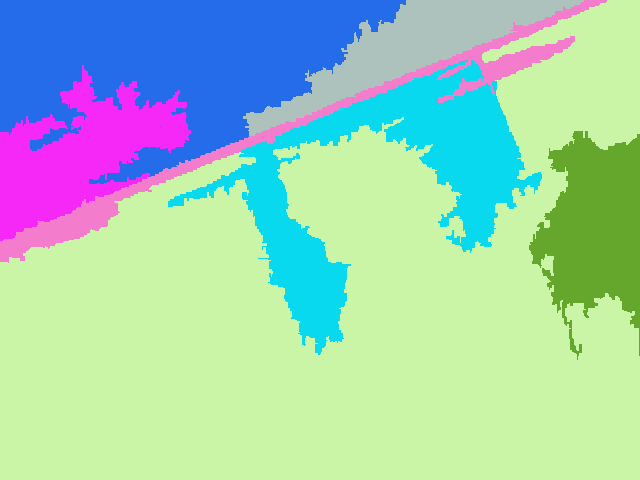
\includegraphics[width=\linewidth]{imgs/seg_srm}
			\caption{SRM}
		\end{subfigure}%
	\end{minipage}
	\caption{Comparação visual de métodos de segmentação}
	\label{fig:comparacaoSegmentacao}
\end{figure}


Adicionalmente, experimentos foram realizados com técnicas de classificação. O objetivo era saber se poderíamos utilizar apenas uma etapa para realizar segmentação e o primeiro nível de classificação. Os resultados foram abaixo do que se consegue na etapa de segmentação isolada. Os resultados foram publicados no \textit{$10^th$ International Conference on Computer Vision Theory and Applications} e o artigo \cite{cavalcanti:2015} completo pode ser visto no apêndice \ref{cap:apendice}.

Para fins de comparação, os resultados deste segundo experimento são apresentados na tabela \ref{tab:experimentoArtigo}. O tempo de execução da classificação para cada imagem no artigo publicado ignora o tempo de extração de características da imagem. Para uma comparação correta com os métodos de segmentação experimentados anteriormente, esse tempo foi acrescido na tabela desta seção.

\begin{table}[h]
\ABNTEXfontereduzida
\centering
\begin{tabulary}{\linewidth}{|L|R|R|}
\hline
\textbf{Algoritmo} & \textbf{Precisão} & \textbf{Tempo/imagem} \\ \hline
Random forest  & 96,0\% & 12,72 s \\ \hline
KNN            & 92,6\% & 22,89 s \\ \hline
Naive Bayes    & 92,8\% & 8,36 s \\ \hline
Decision tree  & 82,2\% & 14,49 s \\ \hline
\end{tabulary}
\caption{Comparação de métodos de classificação para segmentação das imagens em uma única etapa, ordenados por precisão}
\label{tab:experimentoArtigo}
\end{table}


\section{Classificações de regiões}

%TODO realizar experimentos com KNN
%TODO realizar experimentos com SVM
%TODO realizar experimentos com árvores

\section{Próximos passos}

%TODO falar dos experimentos futuros com one-class classifiers

\chapter{Cronograma}

Durante o primeiro ano de estudo, foram cursadas todas as disciplinas e feitas revisões bibliográficas. Também foram realizados os primeiros experimentos com extração de características, segmentação e classificação de terreno (Tabela \ref{tab:atividades2014}). Os próximos passos incluem uma melhora na base de treinamento, revisão das características utilizadas para a detecção de anomalias e realização dos experimentos de detecção dessas anomalias, submissão de artigos junto à comunidade científica e confecção da dissertação de mestrado (Tabela \ref{tab:atividades2015}).

\begin{table}[h]
\resizebox{\textwidth}{!}{%
\begin{tabular}{|l|c|c|c|c|c|c|c|c|c|c|c|c|}
\hline
Atividade/Mês & 02/14 & 03/14 & 04/14 & 05/14 & 06/14 & 07/14 & 08/14 & 09/14 & 10/14 & 11/14 & 12/14 & 01/14 \\ \hline
Disciplinas & \cellcolor{blue!25} & \cellcolor{blue!25} & \cellcolor{blue!25} & \cellcolor{blue!25} & \cellcolor{blue!25} & \cellcolor{blue!25} & \cellcolor{blue!25} & \cellcolor{blue!25} & \cellcolor{blue!25} & \cellcolor{blue!25} & \cellcolor{blue!25} & \cellcolor{blue!25} \\ \hline
Levantamento &  &  &  & \cellcolor{blue!25} & \cellcolor{blue!25} & \cellcolor{blue!25} & \cellcolor{blue!25} &  &  &  &  &  \\ \hline
Experimentos &  &  &  &  &  &  & \cellcolor{blue!25} & \cellcolor{blue!25} & \cellcolor{blue!25} & \cellcolor{blue!25} & \cellcolor{blue!25} & \cellcolor{blue!25} \\ \hline
\end{tabular}
}
\caption{Atividades realizadas em 2014}
\label{tab:atividades2014}
\end{table}

\begin{table}[h]
\resizebox{\textwidth}{!}{%
\begin{tabular}{|l|c|c|c|c|c|c|c|c|c|c|c|c|}
\hline
Atividade/Mês & 02/15 & 03/15 & 04/15 & 05/15 & 06/15 & 07/15 & 08/15 & 09/15 & 10/15 & 11/15 & 12/15 & 01/16 \\ \hline
Experimentos & \cellcolor{blue!25} & \cellcolor{blue!25} & \cellcolor{blue!25} & \cellcolor{blue!25} & \cellcolor{blue!25} & \cellcolor{blue!25} & \cellcolor{blue!25} & & & & & \\ \hline
Sub. de artigos & & & & \cellcolor{blue!25} & \cellcolor{blue!25} & \cellcolor{blue!25} & \cellcolor{blue!25} &  &  &  &  &  \\ \hline
Dissertação &  &  &  & \cellcolor{blue!25} & \cellcolor{blue!25} & \cellcolor{blue!25} & \cellcolor{blue!25} & \cellcolor{blue!25} & \cellcolor{blue!25} & \cellcolor{blue!25} & & \\ \hline
\end{tabular}
}
\caption{Cronograma de atividades para 2015}
\label{tab:atividades2015}
\end{table}

\bibliography{dissertacao}

\apendices

\partapendices

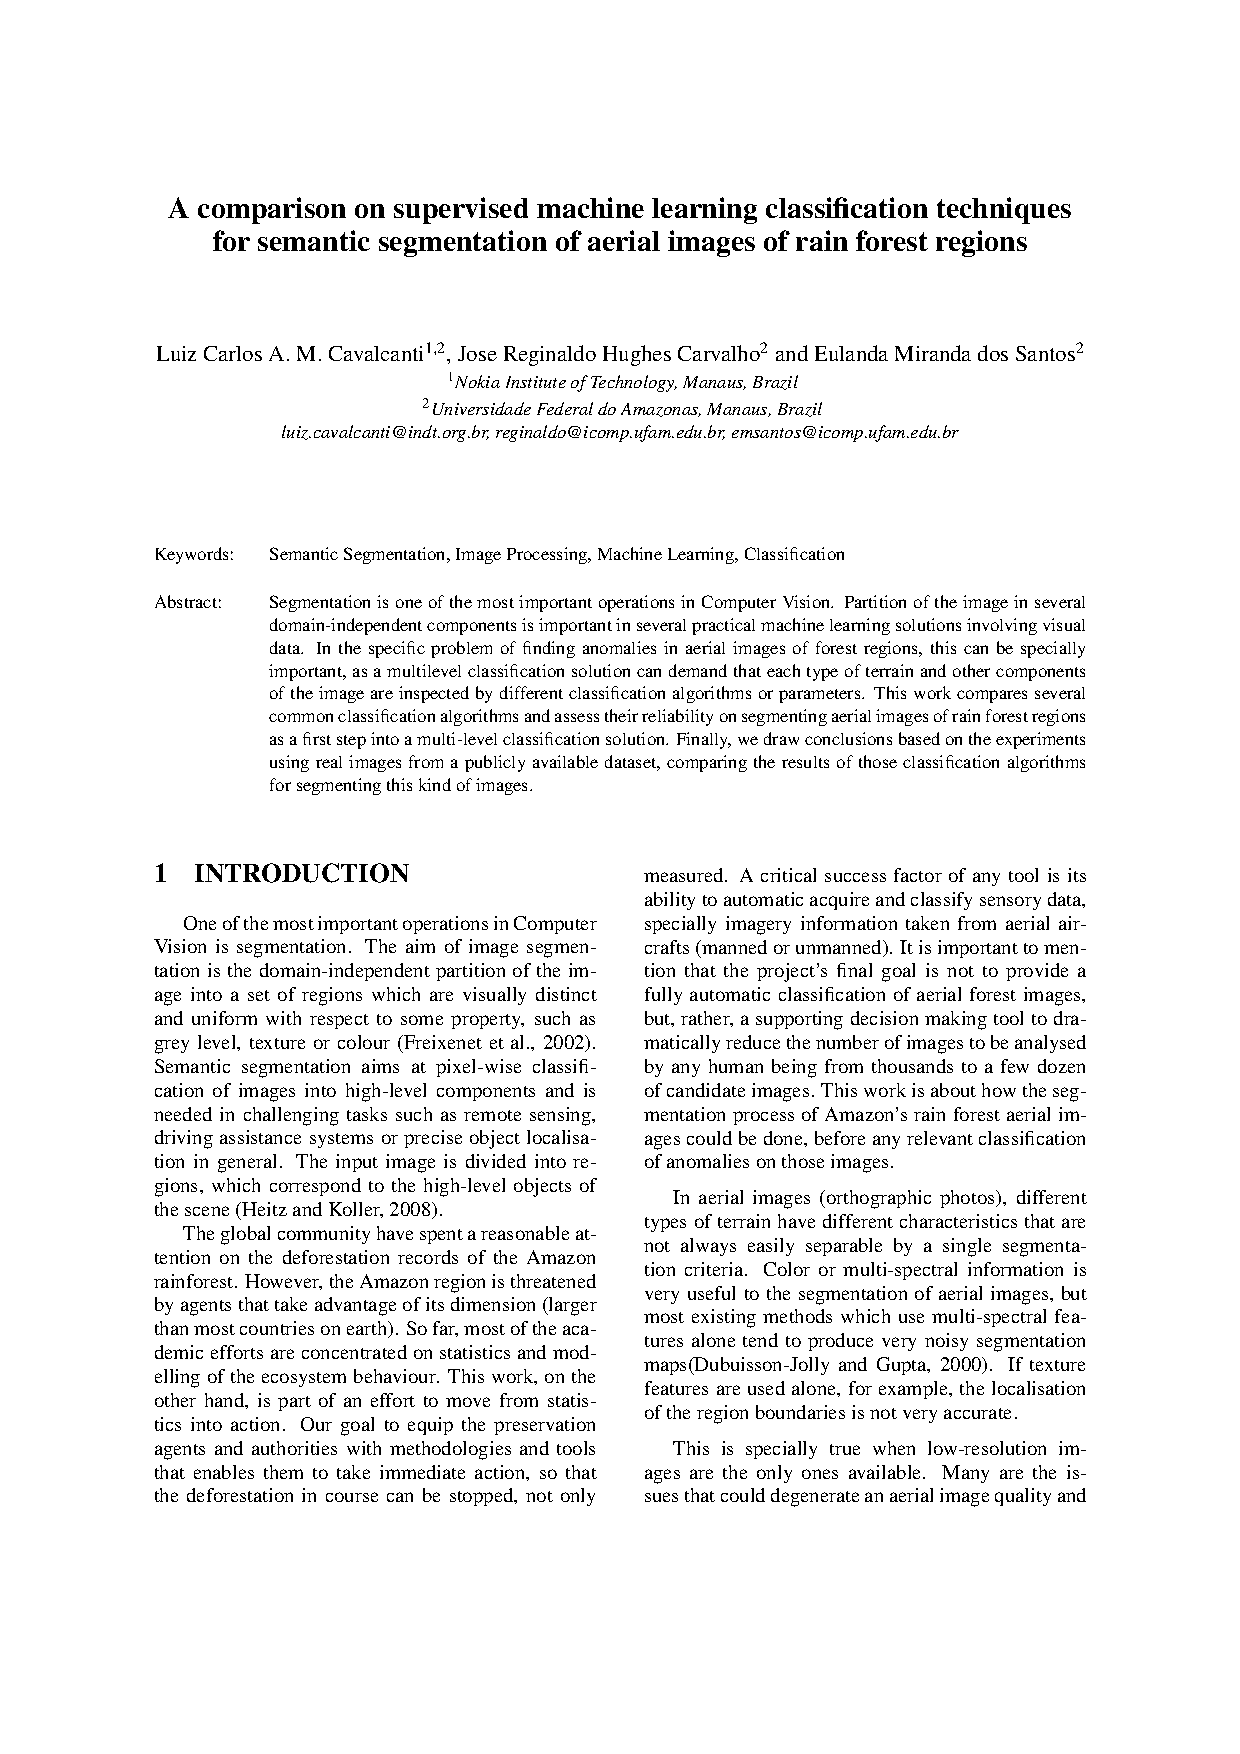
\includepdf[pages={-},addtotoc={1,chapter,1,A comparison on supervised machine learning classification techniques for semantic segmentation of aerial images of rain forest regions,anexo1}]{articles/visapp2015.pdf}

\end{document}
